% KPot v2.0 Research Slides
% New BSD License
% ---------------

% Copyright © 2019 Lilly Chalupowski (lillypad.github.io) All rights reserved.

% Redistribution and use in source and binary forms, with or without modification,
% are permitted provided that the following conditions are met:
% * Redistributions of source code must retain the above copyright notice, this
%   list of conditions and the following disclaimer.
% * Redistributions in binary form must reproduce the above copyright notice, this
%   list of conditions and the following disclaimer in the documentation and/or
%   other materials provided with the distribution.
% * Neither the name of Lilly Chalupowski nor the names of its contributors may be used to
%   endorse or promote products derived from this software without specific prior
%   written permission.

% THIS SOFTWARE IS PROVIDED BY THE COPYRIGHT HOLDERS AND CONTRIBUTORS “AS IS” AND
% ANY EXPRESS OR IMPLIED WARRANTIES, INCLUDING, BUT NOT LIMITED TO, THE IMPLIED
% WARRANTIES OF MERCHANTABILITY AND FITNESS FOR A PARTICULAR PURPOSE ARE
% DISCLAIMED. IN NO EVENT SHALL THE COPYRIGHT OWNER OR CONTRIBUTORS BE LIABLE FOR
% ANY DIRECT, INDIRECT, INCIDENTAL, SPECIAL, EXEMPLARY, OR CONSEQUENTIAL DAMAGES
% (INCLUDING, BUT NOT LIMITED TO, PROCUREMENT OF SUBSTITUTE GOODS OR SERVICES;
% LOSS OF USE, DATA, OR PROFITS; OR BUSINESS INTERRUPTION) HOWEVER CAUSED AND ON
% ANY THEORY OF LIABILITY, WHETHER IN CONTRACT, STRICT LIABILITY, OR TORT
% (INCLUDING NEGLIGENCE OR OTHERWISE) ARISING IN ANY WAY OUT OF THE USE OF THIS
% SOFTWARE, EVEN IF ADVISED OF THE POSSIBILITY OF SUCH DAMAGE.

\documentclass[aspectratio=169]{beamer}
\usepackage{tabularx}
\usepackage{graphicx}
\usepackage{eso-pic}
\usepackage{minted}
\usepackage{hyperref}
\usepackage{tcolorbox}
\usepackage[absolute,overlay]{textpos}

\makeatletter
\newenvironment{myitemize}{%
  \setlength{\topsep}{0pt}
  \setlength{\partopsep}{0pt}
  \renewcommand*{\@listi}{\leftmargin\leftmargini \parsep\z@ \topsep\z@ \itemsep\z@}
  \let\@listI\@listi
  \itemize
}{\enditemize}
\makeatother

\graphicspath{{img/}}

\usetheme{Warsaw}
\usemintedstyle{monokai}

\setbeamercolor{normal text}{fg=white,bg=black!90}
\setbeamercolor{structure}{fg=white}
\setbeamercolor{alerted text}{fg=red!85!black}
\setbeamercolor{item projected}{use=item,fg=black,bg=item.fg!35}
\setbeamercolor*{palette primary}{use=structure,fg=structure.fg}
\setbeamercolor*{palette secondary}{use=structure,fg=structure.fg!95!black}
\setbeamercolor*{palette tertiary}{use=structure,fg=structure.fg!90!black}
\setbeamercolor*{palette quaternary}{use=structure,fg=structure.fg!95!black,bg=black!80}
\setbeamercolor*{framesubtitle}{fg=white}
\setbeamercolor*{block title}{parent=structure,bg=black!60}
\setbeamercolor*{block body}{fg=black,bg=black!10}
\setbeamercolor*{block title alerted}{parent=alerted text,bg=black!15}
\setbeamercolor*{block title example}{parent=example text,bg=black!15}
\setbeamertemplate{navigation symbols}{}
\setbeamercolor{footercolor}{fg=white,bg=black}

\makeatletter
\defbeamertemplate*{footline}{myfootline}
{
  \leavevmode%
  \hbox{%
    \begin{beamercolorbox}[wd=.333333\paperwidth,ht=2.25ex,dp=1ex,center]{footercolor}%
      \insertshorttitle
    \end{beamercolorbox}%
    \begin{beamercolorbox}[wd=.333333\paperwidth,ht=2.25ex,dp=1ex,center]{footercolor}%
      \insertshortauthor\expandafter\beamer@ifempty\expandafter{\beamer@shortinstitute}{}{~~(\insertshortinstitute)}
    \end{beamercolorbox}%
    \begin{beamercolorbox}[wd=.333333\paperwidth,ht=2.25ex,dp=1ex,right]{footercolor}%
      \insertshortdate{}\hspace*{2em}
      \insertframenumber{} / \inserttotalframenumber\hspace*{2ex} 
    \end{beamercolorbox}}%
  \vskip0pt%
}
\makeatother

\title{Finders Keepers (KPot Stealers)}

\institute{GoSecure}
\author{Lilly Chalupowski}
\date{November 15, 2019}

\begin{document}

\setbeamertemplate{footline}{}
{\usebackgroundtemplate{
\includegraphics[width=\paperwidth]{finder-keepers-background.png}}%
\begin{frame}[t]
  \begin{textblock*}{15cm}(1.5cm,6cm) % {block width} (coords) 
    \begin{center}
    \textcolor{black}{\Large{\textbf{Finders Keepers \newline (KPot Stealers)}}}
    \end{center}
  \end{textblock*}
\end{frame}
}

\setbeamertemplate{footline}[myfootline]

\newcommand\AtPagemyUpperLeft[1]{\AtPageLowerLeft{%
\put(\LenToUnit{0.74\paperwidth},\LenToUnit{0.92\paperheight}){#1}}}
\AddToShipoutPictureFG{
  \AtPagemyUpperLeft{{
\includegraphics[width=4cm,keepaspectratio]{gosecure-logo}}}
}%

{\usebackgroundtemplate{
\includegraphics[width=\paperwidth]{question-mark-background.png}}%
\begin{frame}
  \frametitle{whois lilly.chalupowski}
  \begin{table}
    \caption{\textit{who.is results}}
    \begin{tabularx}{\textwidth}{|X|X|}
      \hline
      Name & Lilly Chalupowski \\
      \hline
      Status & Employed \\
      \hline
      Creation Date & 1986 \\
      \hline
      Expiry & A Long Time from Now (Hopefully)\\
      \hline
      Registrant Name & GoSecure \\
      \hline
      Administrative Contact & Travis Barlow \\
      \hline
      Job & TITAN Malware Research Lead \\
      \hline
    \end{tabularx}
  \end{table}
\end{frame}
}

\begin{frame}
  \frametitle{Agenda}
  \framesubtitle{What will we cover?}
  \begin{columns}[onlytextwidth]
    \begin{column}{.50\textwidth}
      \begin{itemize}
      \item{Disclaimer}
      \item{Reverse Engineering}
      \item{Tools of the Trade}
      \item{Injection Techniques}
      \item{Operation Lawyer Loot}
      \end{itemize}
    \end{column}
    \hfill
    \begin{column}{.50\textwidth}
      \begin{center}
        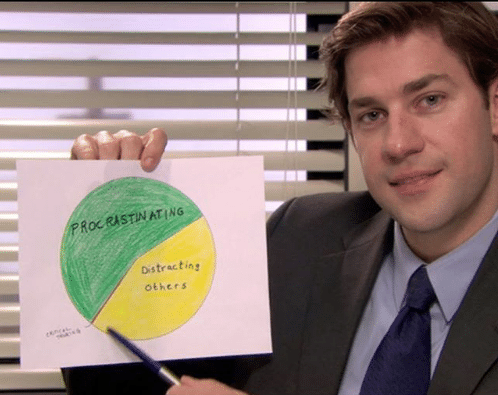
\includegraphics[scale=1.8]{agenda-meme}
      \end{center}
    \end{column}
  \end{columns}
\end{frame}

\begin{frame}
  \frametitle{Disclaimer}
  \framesubtitle{Don't be a Criminal}
  \begin{tcolorbox}[title=disclaimer\_0.log,colback=gray]
    The tools and techniques covered in this presentation can be dangerous and are\\
    being shown for educational purposes.\\
    \newline
    It is a violation of Federal laws to attempt gaining unauthorized access to information, assets or systems belonging to others, or to exceed authorization on systems for which you have not been granted.\\
    \newline
    Only use these tools with/on systems you own or have written permission from the owner. I (the speaker) do not assume any responsibility and shall not be held liable for any illegal use of these tools.\\
  \end{tcolorbox}
\end{frame}

\begin{frame}
  \frametitle{Disclaimer}
  \framesubtitle{Don't be a Fool}
  \begin{tcolorbox}[title=disclaimer\_1.log,colback=gray]
    I (the speaker) do not assume any responsibility and shall not be held
    liable for anyone who infects their machine with the malware discussed in
    this talk. \\
    \newline
    If you need help on preventing the infection of your host machine please
    speak to someone for assistance before you run anything. \\
    \newline
    The malware discussed in this talk can steal your data and more. \\
  \end{tcolorbox}
\end{frame}

\begin{frame}
  \frametitle{Inspiration}
  \framesubtitle{John F. Kennedy}
  \begin{tcolorbox}[title=john\_f\_kennedy.log,colback=gray]
    We choose to reverse engineer! We choose to reverse
    engineer... We choose to reverse engineer and do the other things, not
    because they are easy, but because they are hard; because that goal will
    serve to organize and measure the best of our energies and skills, because
    that challenge is one that we are willing to accept, one we are unwilling to
    postpone, and one we intend to win, and the others, too. - John F. Kennedy \\
  \end{tcolorbox}
\end{frame}

\begin{frame}
  \frametitle{Reverse Engineering}
  \begin{center}
    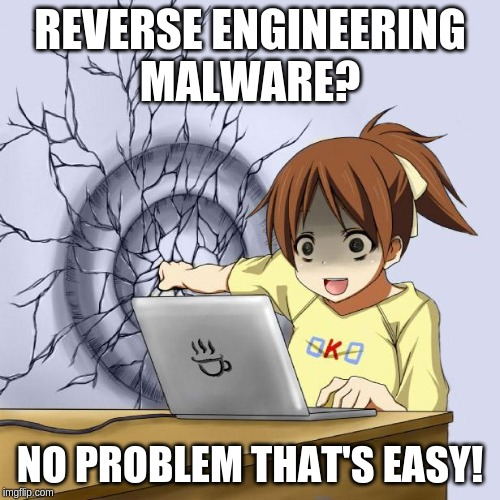
\includegraphics[scale=0.4]{reverse-engineering}
  \end{center}
\end{frame}

\begin{frame}
  \frametitle{Registers}
  \framesubtitle{reverse\_engineering}
  \begin{columns}
    \begin{column}{.50\textwidth}
      \begin{itemize}
      \item{EAX - Return Value of Functions}
      \item{EBX - Base Index (for use with arrays)}
      \item{ECX - Counter in Loops}
      \item{EDI - Destination Memory Operations}
      \item{ESI - Source Memory Operations}
      \item{ESP - Stack Pointer}
      \item{EBP - Base Frame Pointer}
      \end{itemize}
    \end{column}
    \hfill
    \begin{column}{.50\textwidth}
      \begin{center}
        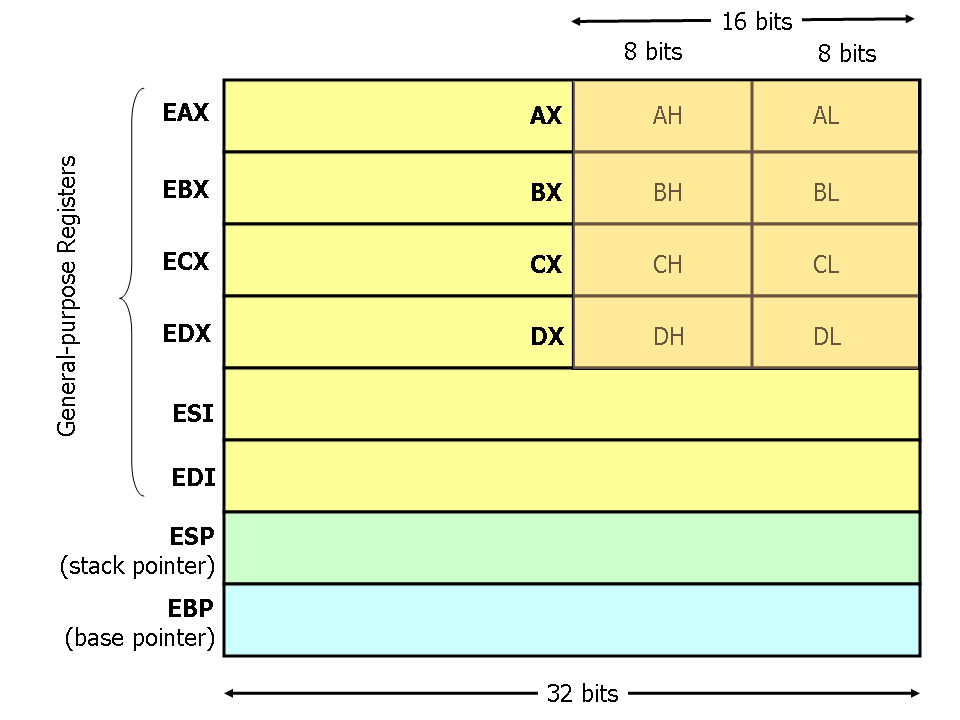
\includegraphics[scale=0.25]{x86-registers}
      \end{center}
    \end{column}
  \end{columns}
  \bigskip
  Did You Know: In computer architecture, a processor register is a quickly accessible location available to a computer's central processing unit (CPU).
\end{frame}

\begin{frame}
  \frametitle{Stack Overview}
  \framesubtitle{reverse\_engineering}
  \begin{columns}
    \begin{column}{.40\textwidth}
      \begin{itemize}
      \item{Last-In First-Out}
      \item{Downward Growth}
      \item{Function Local Variables}
      \item{ESP}
      \item{Increment / Decrement = 4}
        \begin{itemize}
        \item{Double-Word Aligned}
        \end{itemize}
      \end{itemize}
    \end{column}
    \hfill
    \begin{column}{.60\textwidth}
      \begin{center}
        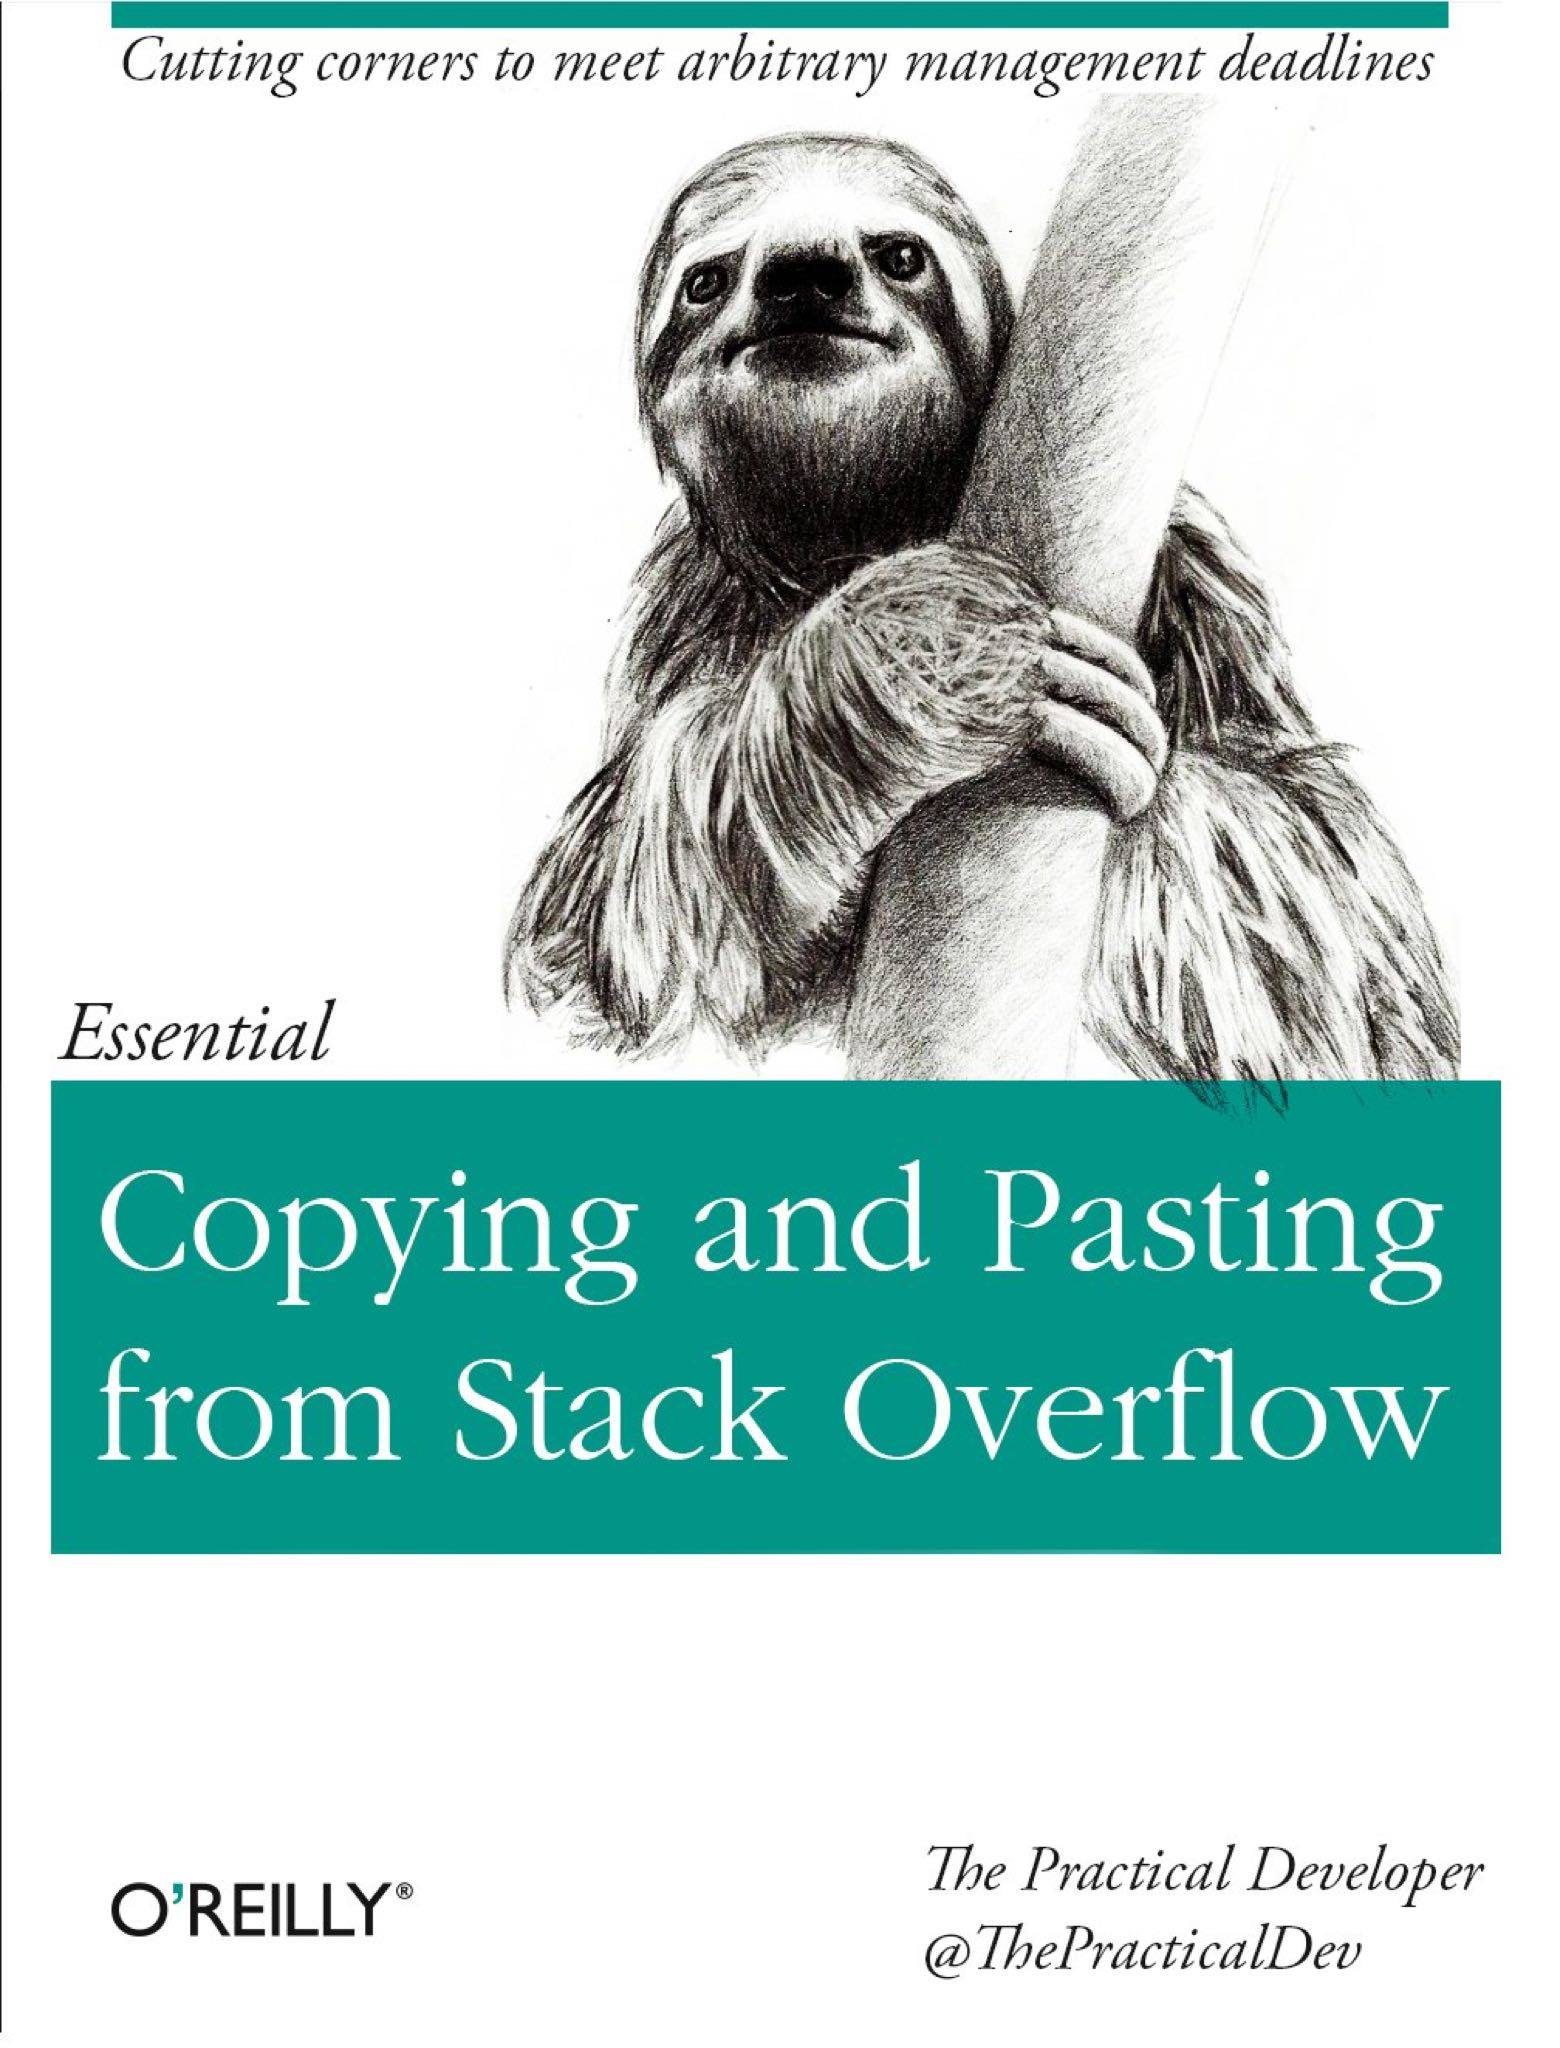
\includegraphics[scale=0.09]{stack-overflow-meme}
      \end{center}
    \end{column}
  \end{columns}
  \end{frame}

\begin{frame}
  \frametitle{Stack Structure}
  \framesubtitle{reverse\_engineering}
  \begin{center}
    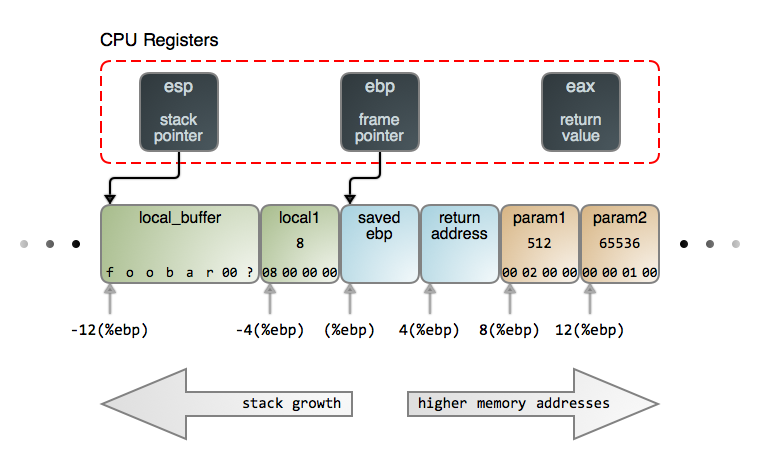
\includegraphics[scale=0.42]{the-stack}
  \end{center}
\end{frame}

\begin{frame}
  \frametitle{Control Flow}
  \framesubtitle{reverse\_engineering}
  \begin{columns}
    \begin{column}{.5\textwidth}
      \begin{itemize}
        \item{Conditionals}
          \begin{itemize}
          \item{CMP}
            % Compares both operands by subtraction to determine if the result
            % is 0
          \item{TEST}
           % [TEST] computes the bit-wise logical AND of first operand (source 1 operand) and the second operand (source 2 operand) and sets the SF, ZF, and PF status flags according to the result. 
           % A	 	B	 	C
           % 0	 AND 	0	->	0
           % 0	 AND 	1	->	0
           % 1	 AND 	0	->	0
           % 1	 AND 	1	->	1
          \item{JMP}
          % Jumps to the specified address
          \item{JNE}
          \item{JNZ}
          \end{itemize}
      \item{EFLAGS}
        \begin{itemize}
        \item{ZF / Zero Flag}
          % Set if the result of the previous arithmetic operation is zero
        \item{SF / Sign Flag}
          % Set to the most significant bit of the result
          % Alternatively referred to as the alt bit, high bit, meta bit, or senior bit the most significant bit is the highest bit in a series of numbers in binary, located at the far left of a string. For example, in the number 01001001, the most significant bit is the 0 at the beginning of the line.
        \item{CF / Carry Flag}
          % Set when the result requires a carry. It applies to unsigned numbers
        \item{OF/Overflow Flag}
          % Set if the result overflows the max size. It applies to signed numbers
        \end{itemize}
      \end{itemize}
    \end{column}
    \hfill
    \begin{column}{.5\textwidth}
      \begin{center}
        
\includegraphics[scale=0.25]{zero-flag-meme}
      \end{center}
    \end{column}
  \end{columns}
\end{frame}

\begin{frame}
  \frametitle{Calling Conventions}
  \framesubtitle{reverse\_engineering}
  \begin{columns}
    \begin{column}{.5\textwidth}
      \begin{itemize}
      \item{CDECL}
        \begin{itemize}
        \item{Arguments Right-to-Left}
        \item{Return Values in EAX}
        \item{Caller Function Cleans the Stack}
        \end{itemize}
      \item{STDCALL}
        \begin{itemize}
        \item{Used in Windows Win32API}
        \item{Arguments Right-to-Left}
        \item{Return Values in EAX}
        \item{The Callee function cleans the stack, unlike CDECL}
        \item{Does not support variable arguments}
        \end{itemize}
      \item{FASTCALL}
        \begin{itemize}
        \item{Uses registers as arguments}
        \item{Useful for shellcode}
        \end{itemize}
      \end{itemize}
    \end{column}
    \hfill
    \begin{column}{.5\textwidth}
      \begin{center}
        
\includegraphics[scale=0.27]{cdecl-meme}
      \end{center}
    \end{column}
  \end{columns}
\end{frame}

\begin{frame}
  \frametitle{Windows Memory Structure}
  \framesubtitle{reverse\_engineering}
  \begin{columns}
    \begin{column}{.6\textwidth}
      \begin{itemize}
      \item{Stack - Grows up to lower addresses}
      \item{Heap - Grows down to higher addresses}
      \item{Program Image}
      \item{TEB - Thread Environment Block}
        \begin{itemize}
        \item{GetLastError()}
        \item{GetVersion()}
        \item{Pointer to the PEB}
        \end{itemize}
        % stores information about the currently running thread
        % The TIB can be used to get a lot of information on the process without calling Win32 API. Examples include emulating GetLastError(), GetVersion(). Through the pointer to the PEB one can obtain access to the import tables (IAT), process startup arguments, image name, etc. It is accessed from the FS segment register when operating on 32 bits, and from GS in 64 bits.
      \item{PEB - Process Environment Block}
        \begin{itemize}
        \item{Image Name}
        \item{Global Context}
        \item{Startup Parameters}
        \item{Image Base Address}
        \item{IAT (Import Address Table)}
        \end{itemize}
        % The PEB contains data structures that apply across a whole process, including global context, startup parameters, data structures for the program image loader, the program image base address, and synchronization objects used to provide mutual exclusion for process-wide data structures. 
      \end{itemize}
    \end{column}
    \hfill
    \begin{column}{.7\textwidth}
      \begin{center}
        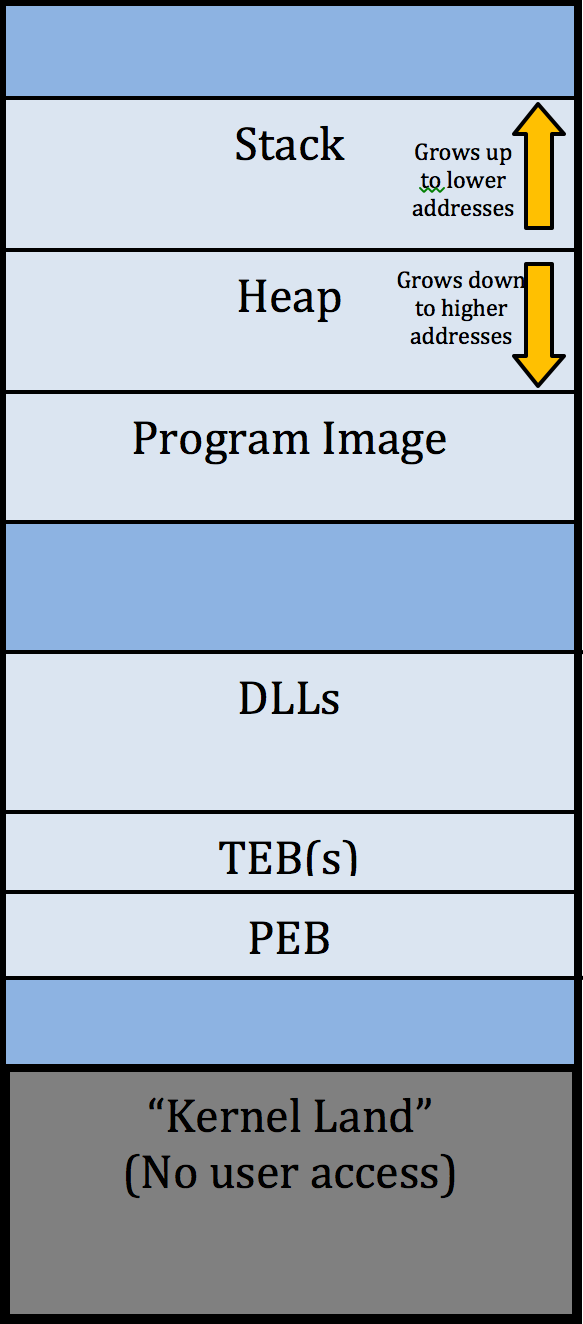
\includegraphics[scale=0.30]{the-heap}
      \end{center}
    \end{column}
  \end{columns}
\end{frame}

\begin{frame}
  \frametitle{IAT and IDT}
  \framesubtitle{reverse\_engineering}
  \begin{columns}
    \begin{column}{.4\textwidth}
      \begin{itemize}
        \item{Identical to the IDT (Import Directory Table)}
        \item{Binding - The process of where functions are mapped to their
            virtual addresses overwriting the IAT}
        \item{Often the IDT and IAT must be rebuilt when packing and unpacking malware}
      \end{itemize}
    \end{column}
    \hfill
    \begin{column}{.6\textwidth}
      \begin{center}
        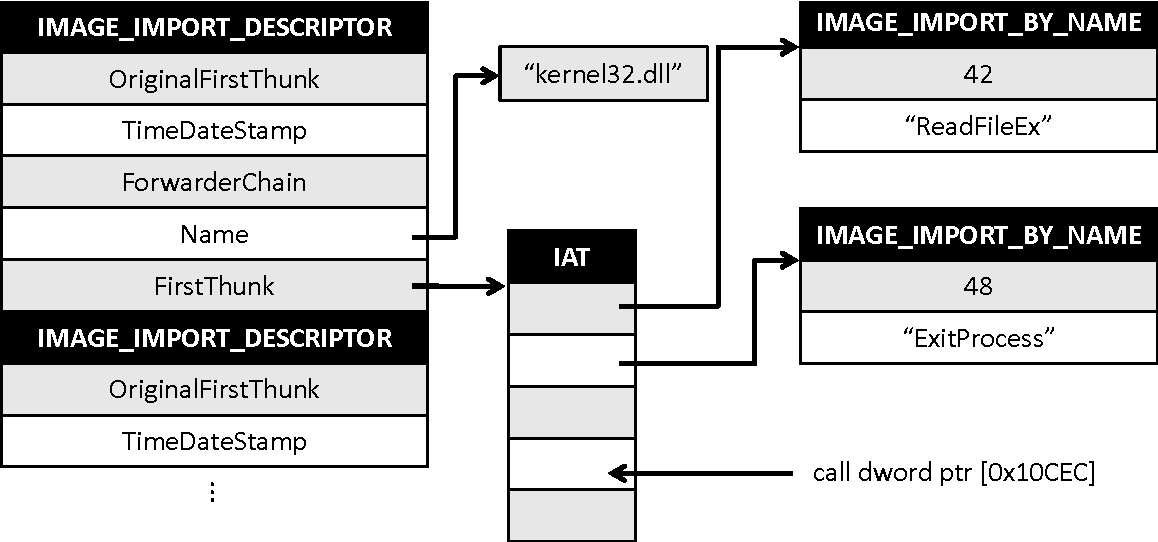
\includegraphics[scale=0.2]{IAT}
      \end{center}
    \end{column}
  \end{columns}
  % Mapped format is when it's mapped to memory with virtual addresses
  % after loaded by Windows
  % Unmapped is when it uses it's raw addresses before it's loaded into memory
  % by Windows
\end{frame}

\begin{frame}
  \frametitle{Assembly}
  \framesubtitle{reverse\_engineering}
  \begin{columns}
    \begin{column}{.35\textwidth}
      \begin{itemize}
      \item{Common Instructions}
        \begin{itemize}
        \item{MOV}
        \item{LEA}
        \item{XOR}
        \item{PUSH}
        \item{POP}
      \end{itemize}
    \end{itemize}
    \end{column}
    \hfill
    \begin{column}{0.65\textwidth}
      \begin{center}
        
\includegraphics[scale=0.40]{assembly-meme}
      \end{center}
    \end{column}
  \end{columns}
\end{frame}

\begin{frame}[fragile]{}
  \frametitle{Assembly CDECL (Linux)}
  \framesubtitle{reverse\_engineering}
  \begin{center}
    \begin{tcolorbox}[title=cdecl.c,colback=black]
        \begin{minted}[fontsize=\small]{c}
          __cdecl int add_cdecl(int a, int b){
            return a + b;
          }
          int x = add_cdecl(2, 3);
        \end{minted}
    \end{tcolorbox}
  \end{center}
\end{frame}

\begin{frame}[fragile]{}
  \frametitle{Assembly CDECL (Linux)}
  \framesubtitle{reverse\_engineering}
  \begin{center}
    \begin{tcolorbox}[title=cdecl.asm,colback=black]
        \begin{minted}[fontsize=\small]{asm}
          _add_cdecl:
            push ebp
            mov ebp, esp
            mov eax, [ebp + 8]  ; get 3 from the stack
            mov edx, [ebp + 12] ; get 2 from the stack
            add eax, edx        ; add values to eax
            pop ebp
            ret
          _start:
            push 3              ; second argument 
            push 2              ; first argument
            call _add_cdecl
            add esp, 8
        \end{minted}
    \end{tcolorbox}
  \end{center}
\end{frame}

\begin{frame}[fragile]{}
  \frametitle{Assembly STDCALL (Windows)}
  \framesubtitle{reverse\_engineering}
  \begin{center}
    \begin{tcolorbox}[title=stdcall.c,colback=black]
        \begin{minted}[fontsize=\small]{c}
          __stdcall int add_stdcall(int a, int b){
            return a + b;
          }
          int x = add_stdcall(2, 3);
        \end{minted}
    \end{tcolorbox}
  \end{center}
\end{frame}

\begin{frame}[fragile]{}
  \frametitle{Assembly STDCALL (Windows)}
  \framesubtitle{reverse\_engineering}
  \begin{center}
    \begin{tcolorbox}[title=stdcall.asm,colback=black]
        \begin{minted}[fontsize=\small]{asm}
          _add_stdcall:
            push ebp
            mov ebp, esp
            mov eax, [ebp + 8]  ; set eax to 3
            mov edx, [ebp + 12] ; set edx to 2
            add eax, edx
            pop ebp
            ret 8               ; how many bytes to pop
          _start:               ; main function
            push 3              ; second argument
            push 2              ; first argument
            call _add_stdcall
        \end{minted}
        % In the function body, the ret instruction has an (optional) argument that indicates how many bytes to pop off the stack when the function returns.
        % STDCALL functions are name-decorated with a leading underscore, followed by an @, and then the number (in bytes) of arguments passed on the stack. This number will always be a multiple of 4, on a 32-bit aligned machine.
    \end{tcolorbox}
  \end{center}
\end{frame}

\begin{frame}[fragile]{}
  \frametitle{Assembly FASTCALL}
  \framesubtitle{reverse\_engineering}
  \begin{center}
    \begin{tcolorbox}[title=cdecl.c,colback=black]
        \begin{minted}[fontsize=\small]{c}
          __fastcall int add_fastcall(int a, int b){
            return a + b;
          }
          int x = add_fastcall(2, 3);
        \end{minted}
        % The FASTCALL calling convention is not completely standard across all compilers, so it should be used with caution. In FASTCALL, the first 2 or 3 32-bit (or smaller) arguments are passed in registers, with the most commonly used registers being edx, eax, and ecx. Additional arguments, or arguments larger than 4-bytes are passed on the stack, often in Right-to-Left order (similar to CDECL). The calling function most frequently is responsible for cleaning the stack, if needed.
        % Because of the ambiguities, it is recommended that FASTCALL be used only in situations with 1, 2, or 3 32-bit arguments, where speed is essential.
    \end{tcolorbox}
  \end{center}
\end{frame}

\begin{frame}[fragile]{}
  \frametitle{Assembly FASTCALL}
  \framesubtitle{reverse\_engineering}
  \begin{center}
    \begin{tcolorbox}[title=fastcall.asm,colback=black]
        \begin{minted}[fontsize=\small]{asm}
          _add_fastcall:
            push ebp
            mov ebp, esp
            add eax, edx        ; add and save result in eax
            pop ebp
            ret
          _start:
            mov eax, 2          ; first argument
            mov edx, 3          ; second argument
            call _add_fastcall
        \end{minted}
        % In the function body, the ret instruction has an (optional) argument that indicates how many bytes to pop off the stack when the function returns.
        % STDCALL functions are name-decorated with a leading underscore, followed by an @, and then the number (in bytes) of arguments passed on the stack. This number will always be a multiple of 4, on a 32-bit aligned machine.
    \end{tcolorbox}
  \end{center}
\end{frame}


\begin{frame}[fragile]{}
  \frametitle{Guess the Calling Convention}
  \framesubtitle{reverse\_engineering}
  \begin{center}
    \begin{tcolorbox}[title=hello.asm,colback=black]
    \begin{minipage}{0.8\textwidth}
      \begin{minted}[fontsize=\small]{asm}
        section     .text                  ; the code section
        global      _start                 ; tell linker entrypoint
        _start:
          mov     edx,len                  ; message length
          mov     ecx,msg                  ; message to write
          mov     ebx,1                    ; file descriptor stdout
          mov     eax,4                    ; syscall number for write
          int     0x80                     ; linux x86 interrupt
          mov     eax,1                    ; syscall number for exit
          int     0x80                     ; linux x86 interrupt
        section     .data                  ; the data section
          msg     db  'Hello, world!',0x0  ; null terminated string
          len     equ \$ - msg             ; message length
      \end{minted}
    \end{minipage}
    \end{tcolorbox}
  \end{center}
\end{frame}

\begin{frame}
  \frametitle{Assembler and Linking}
  \framesubtitle{reverse\_engineering}
  \begin{center}
    \begin{tcolorbox}[title=terminal,colback=black]
      \begin{minipage}{0.8\textwidth}
        \textbf{\textcolor{green}{malware@work \textcolor{blue}{\~ \$}}} \textcolor{white}{ nasm -f elf32 -o hello.o hello.asm}
        \newline
        \textbf{\textcolor{green}{malware@work \textcolor{blue}{\~ \$}}} \textcolor{white}{ ld -m elf\_i386 -o hello hello.o}
        \newline
        \textbf{\textcolor{green}{malware@work \textcolor{blue}{\~ \$}}} \textcolor{white}{ ./hello}
        \newline
        \textcolor{white}{ Hello, World!}
        \newline
        \textbf{\textcolor{green}{malware@work \textcolor{blue}{\~ \$}}}
      \end{minipage}
    \end{tcolorbox}
  \end{center}
\end{frame}

\begin{frame}
  \frametitle{Assembly Flavors}
  \framesubtitle{reverse\_engineering}
  \begin{center}
    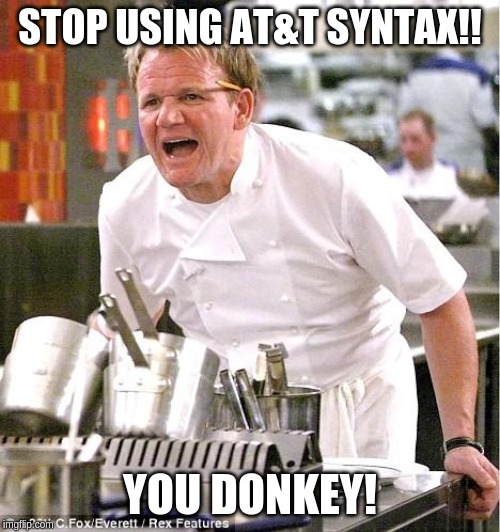
\includegraphics[scale=0.35]{intel-vs-atnt-meme}
  \end{center}
\end{frame}

\begin{frame}
  \frametitle{Tools of the Trade}
  \begin{center}
    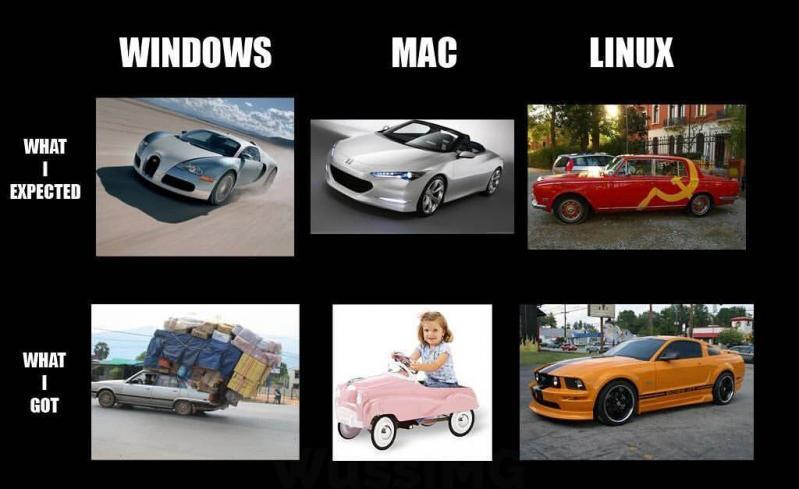
\includegraphics[scale=0.5]{mac-meme}
  \end{center}
\end{frame}

\begin{frame}
  \frametitle{VirtualBox}
  \framesubtitle{tools\_of\_the\_trade}
  \begin{columns}
    \begin{column}{.3\textwidth}
      \begin{itemize}
      \item{Snapshots}
      \item{Security Layer}
      \item{Multiple Systems}
      \end{itemize}
    \end{column}
    \hfill
    \begin{column}{.7\textwidth}
      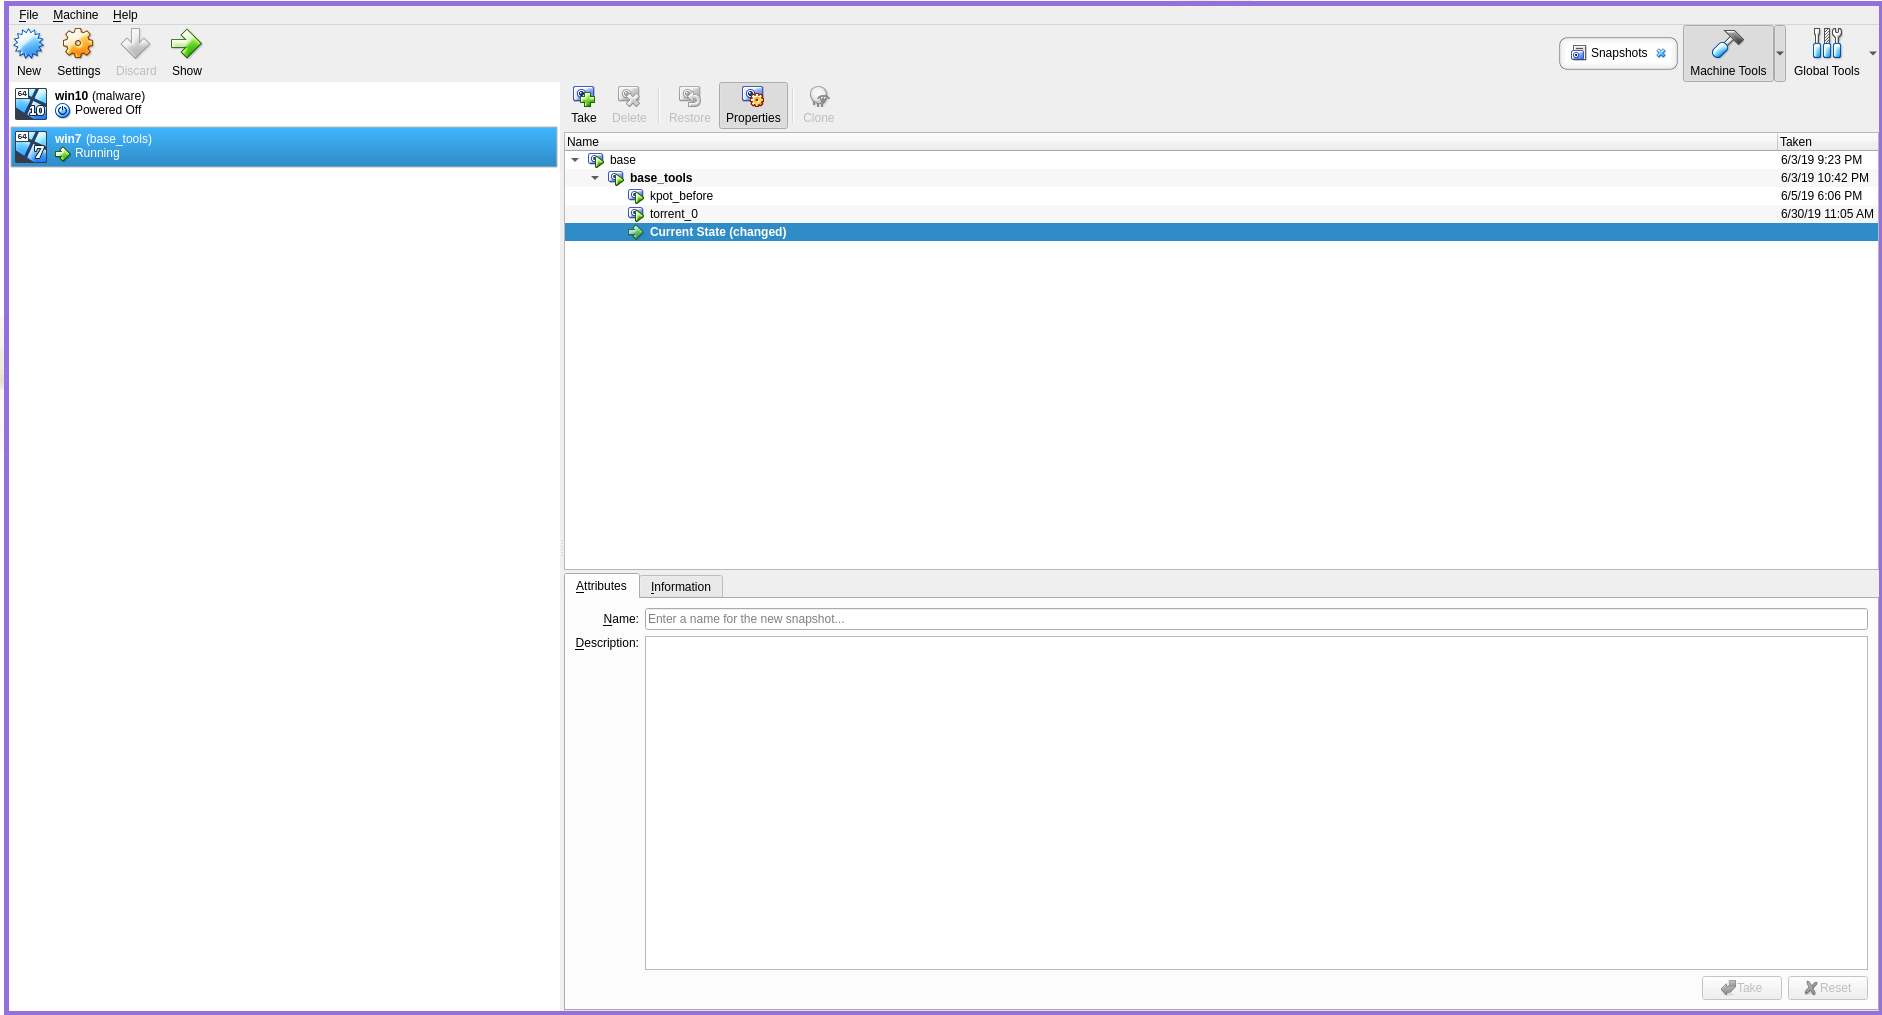
\includegraphics[scale=0.6]{virtualbox}
    \end{column}
  \end{columns}
\end{frame}

\begin{frame}
  \frametitle{x64dbg}
  \framesubtitle{tools\_of\_the\_trade}
  \begin{columns}
    \begin{column}{.3\textwidth}
      \begin{itemize}
      \item{Resolving APIs}
      \item{Dumping Memory}
      \item{Modify Control Flow}
      \item{Identify Key Behaviors}
      \end{itemize}
    \end{column}
    \hfill
    \begin{column}{.7\textwidth}
      \begin{center}
        
\includegraphics[scale=0.5]{stages-of-debugging-meme}
      \end{center}
    \end{column}
  \end{columns}
\end{frame}

\begin{frame}
  \frametitle{x64dbg}
  \framesubtitle{tools\_of\_the\_trade}
  \begin{center}
    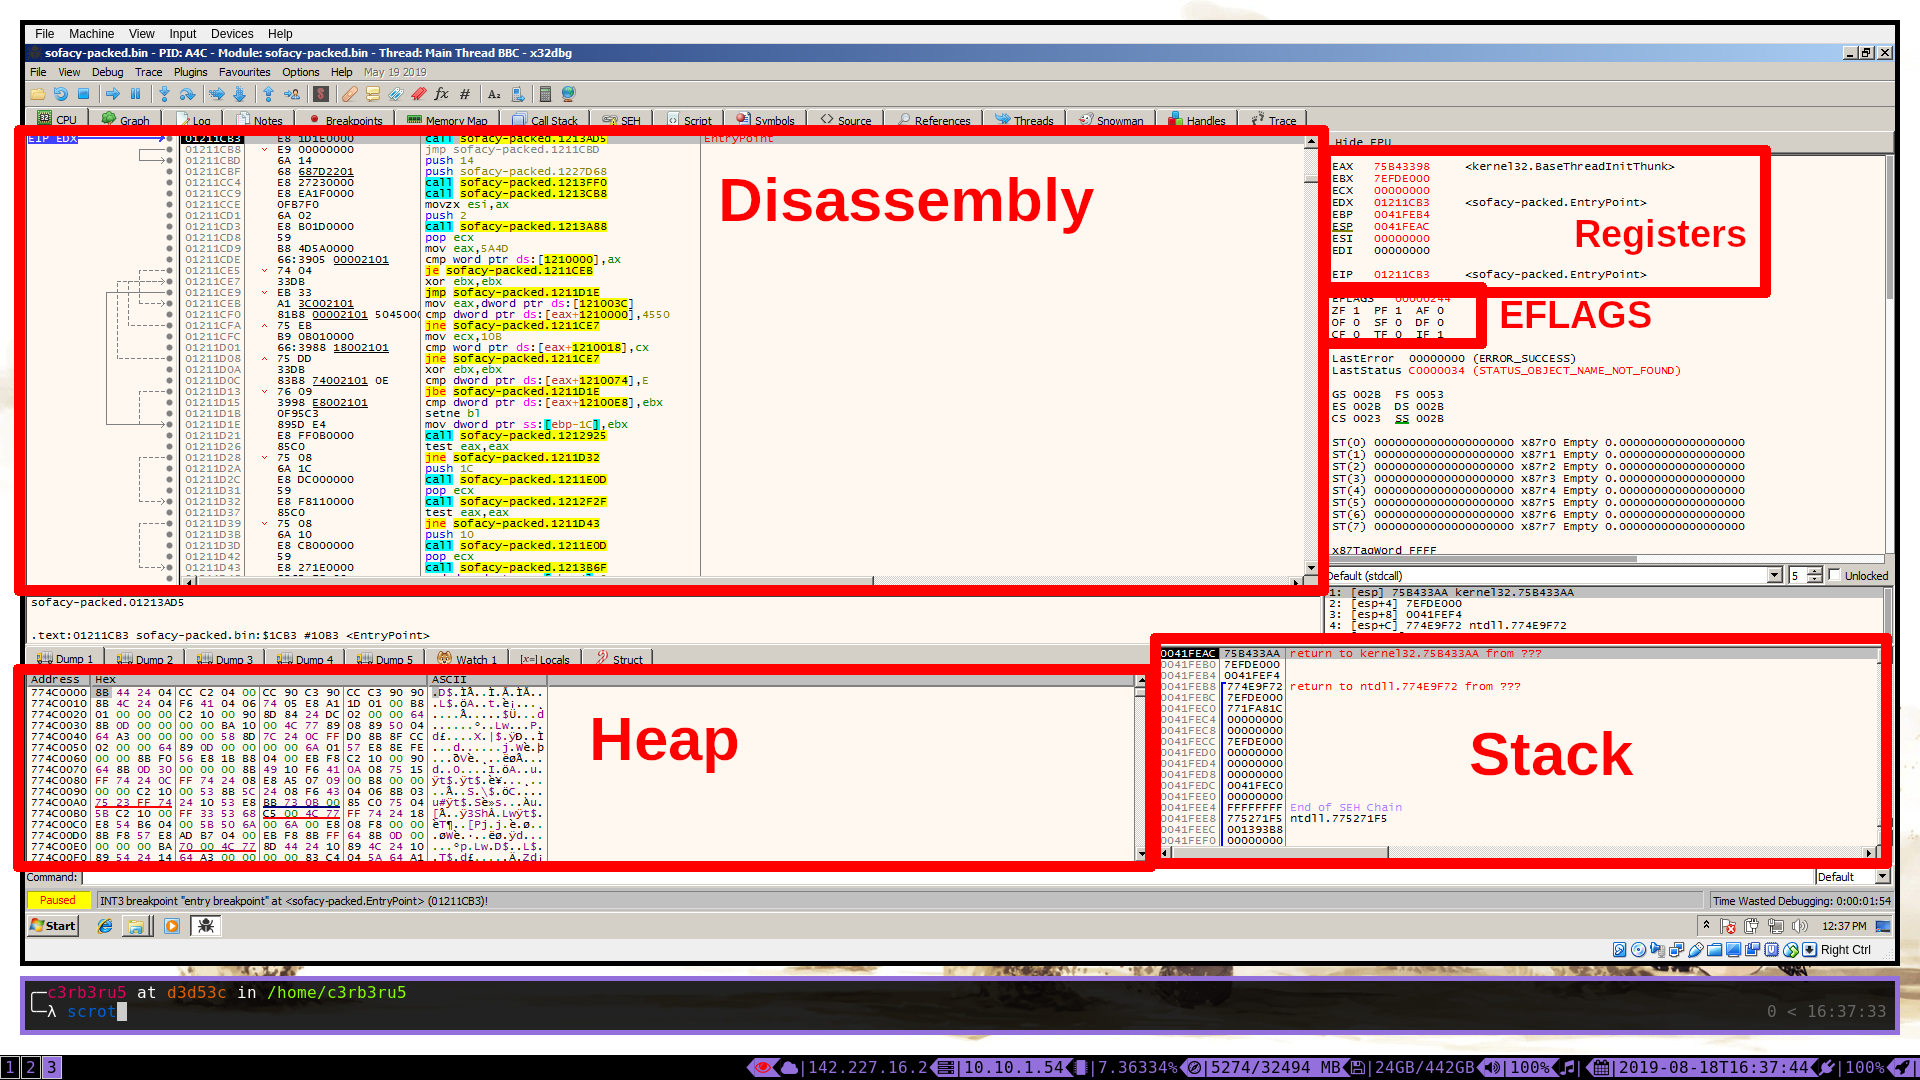
\includegraphics[scale=0.75]{x64dbg-overview}
  \end{center}
\end{frame}

\begin{frame}
  \frametitle{x64dbg}
  \framesubtitle{tools\_of\_the\_trade}
  \begin{center}
    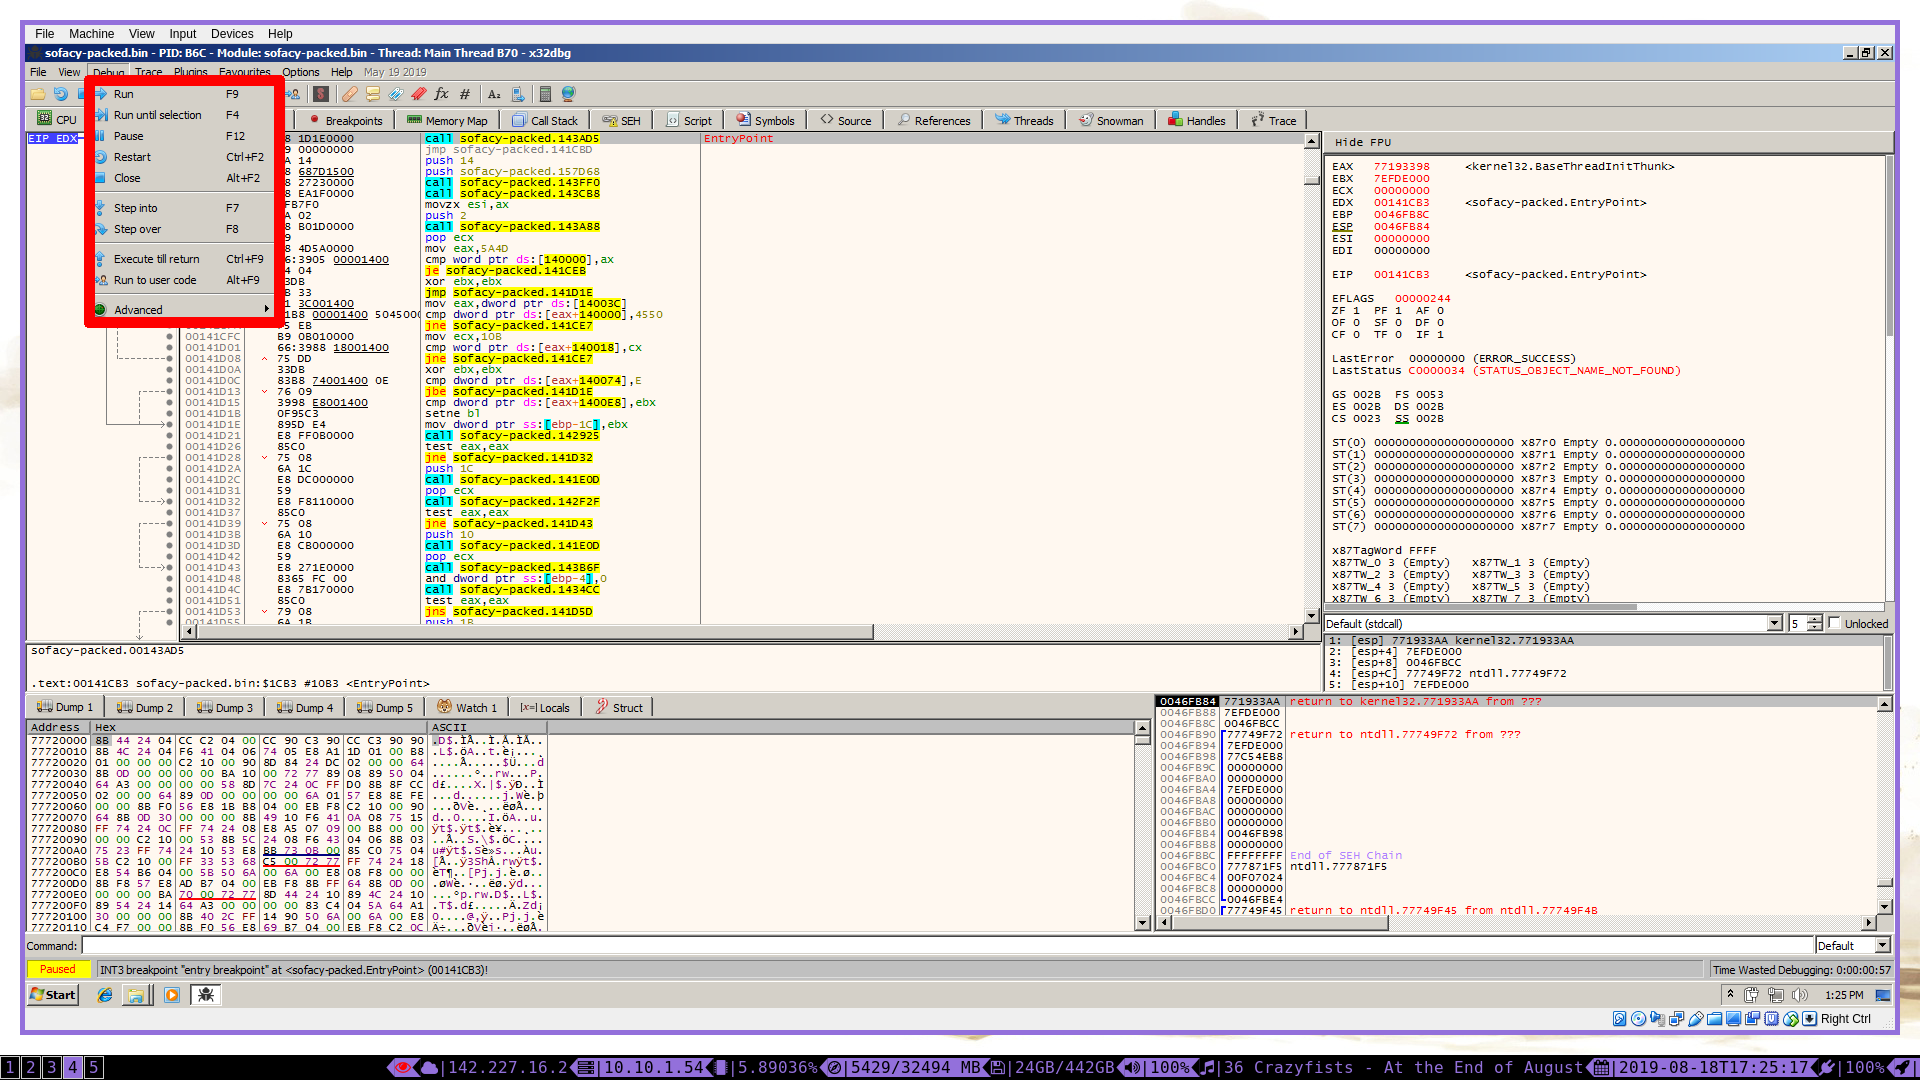
\includegraphics[scale=0.75]{x64dbg-navigation}
  \end{center}
\end{frame}

\begin{frame}
  \frametitle{x64dbg}
  \framesubtitle{tools\_of\_the\_trade}
  \begin{center}
    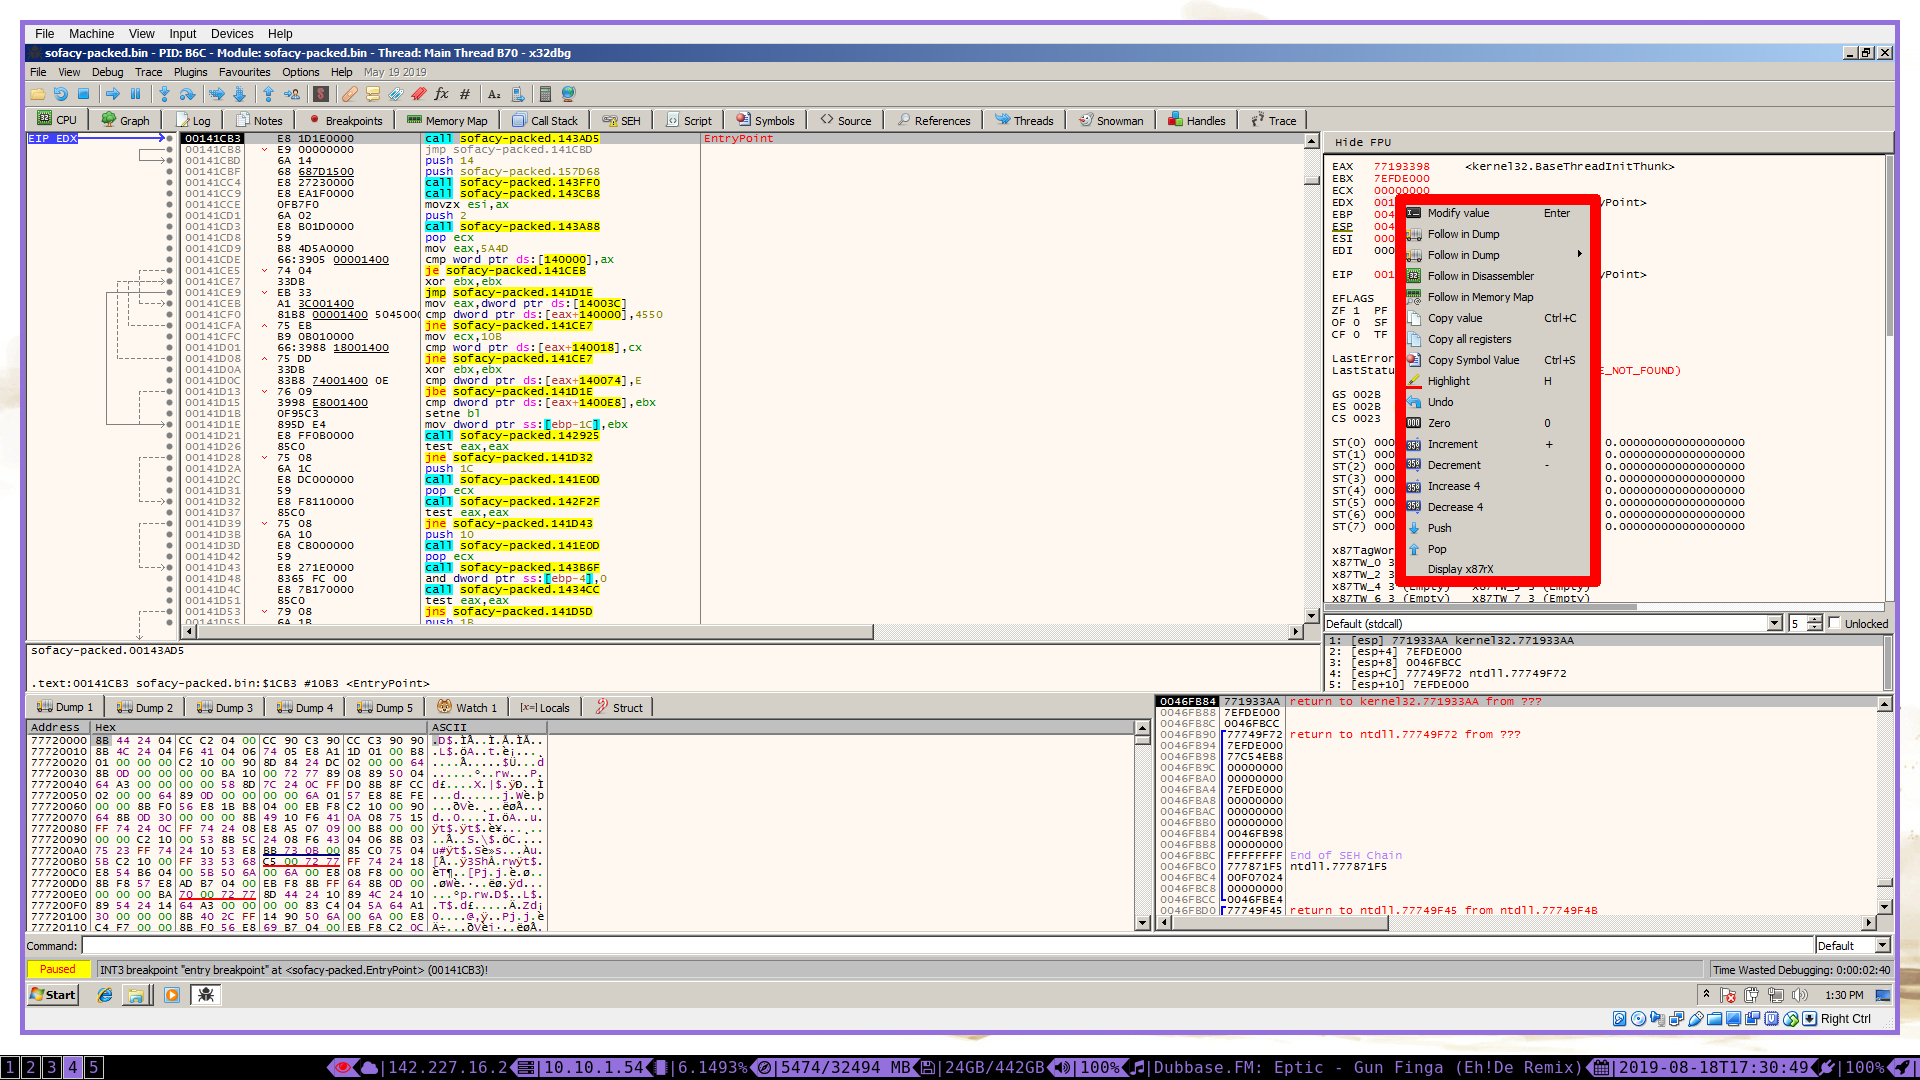
\includegraphics[scale=0.75]{x64dbg-context-menu}
  \end{center}
\end{frame}

\begin{frame}
  \frametitle{Cutter}
  \framesubtitle{tools\_of\_the\_trade}
  \begin{columns}
    \begin{column}{.3\textwidth}
      \begin{itemize}
      \item{Markup Reverse Engineered Code}
      \item{Control Flow Navigation}
      \item{Pseudo Code}
      \end{itemize}
    \end{column}
    \hfill
    \begin{column}{.7\textwidth}
      \begin{center}
        
\includegraphics[scale=0.4]{ida-pro-meme}
      \end{center}
    \end{column}
  \end{columns}
\end{frame}

\begin{frame}
  \frametitle{Cutter}
  \framesubtitle{tools\_of\_the\_trade}
  \begin{center}
    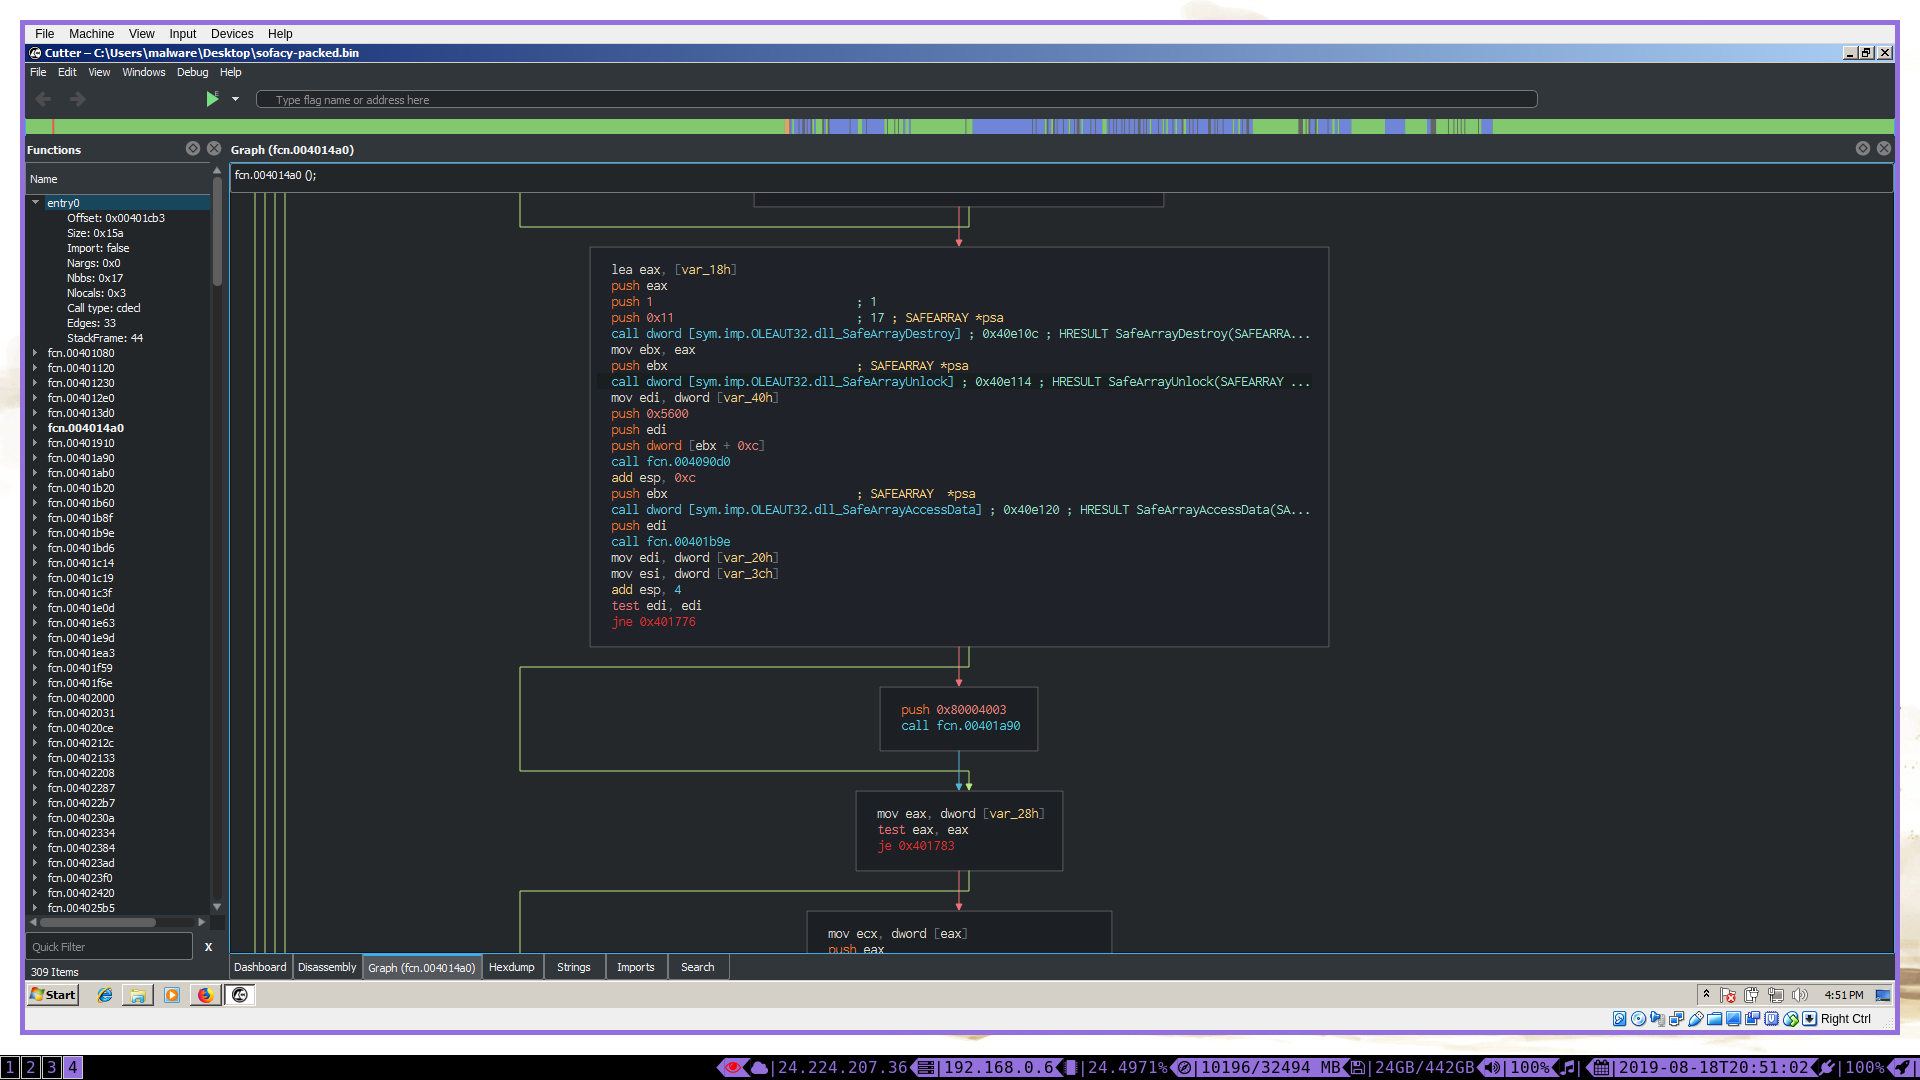
\includegraphics[scale=0.18]{cutter-graph}
  \end{center}
\end{frame}

\begin{frame}
  \frametitle{Cutter}
  \framesubtitle{tools\_of\_the\_trade}
  \begin{center}
    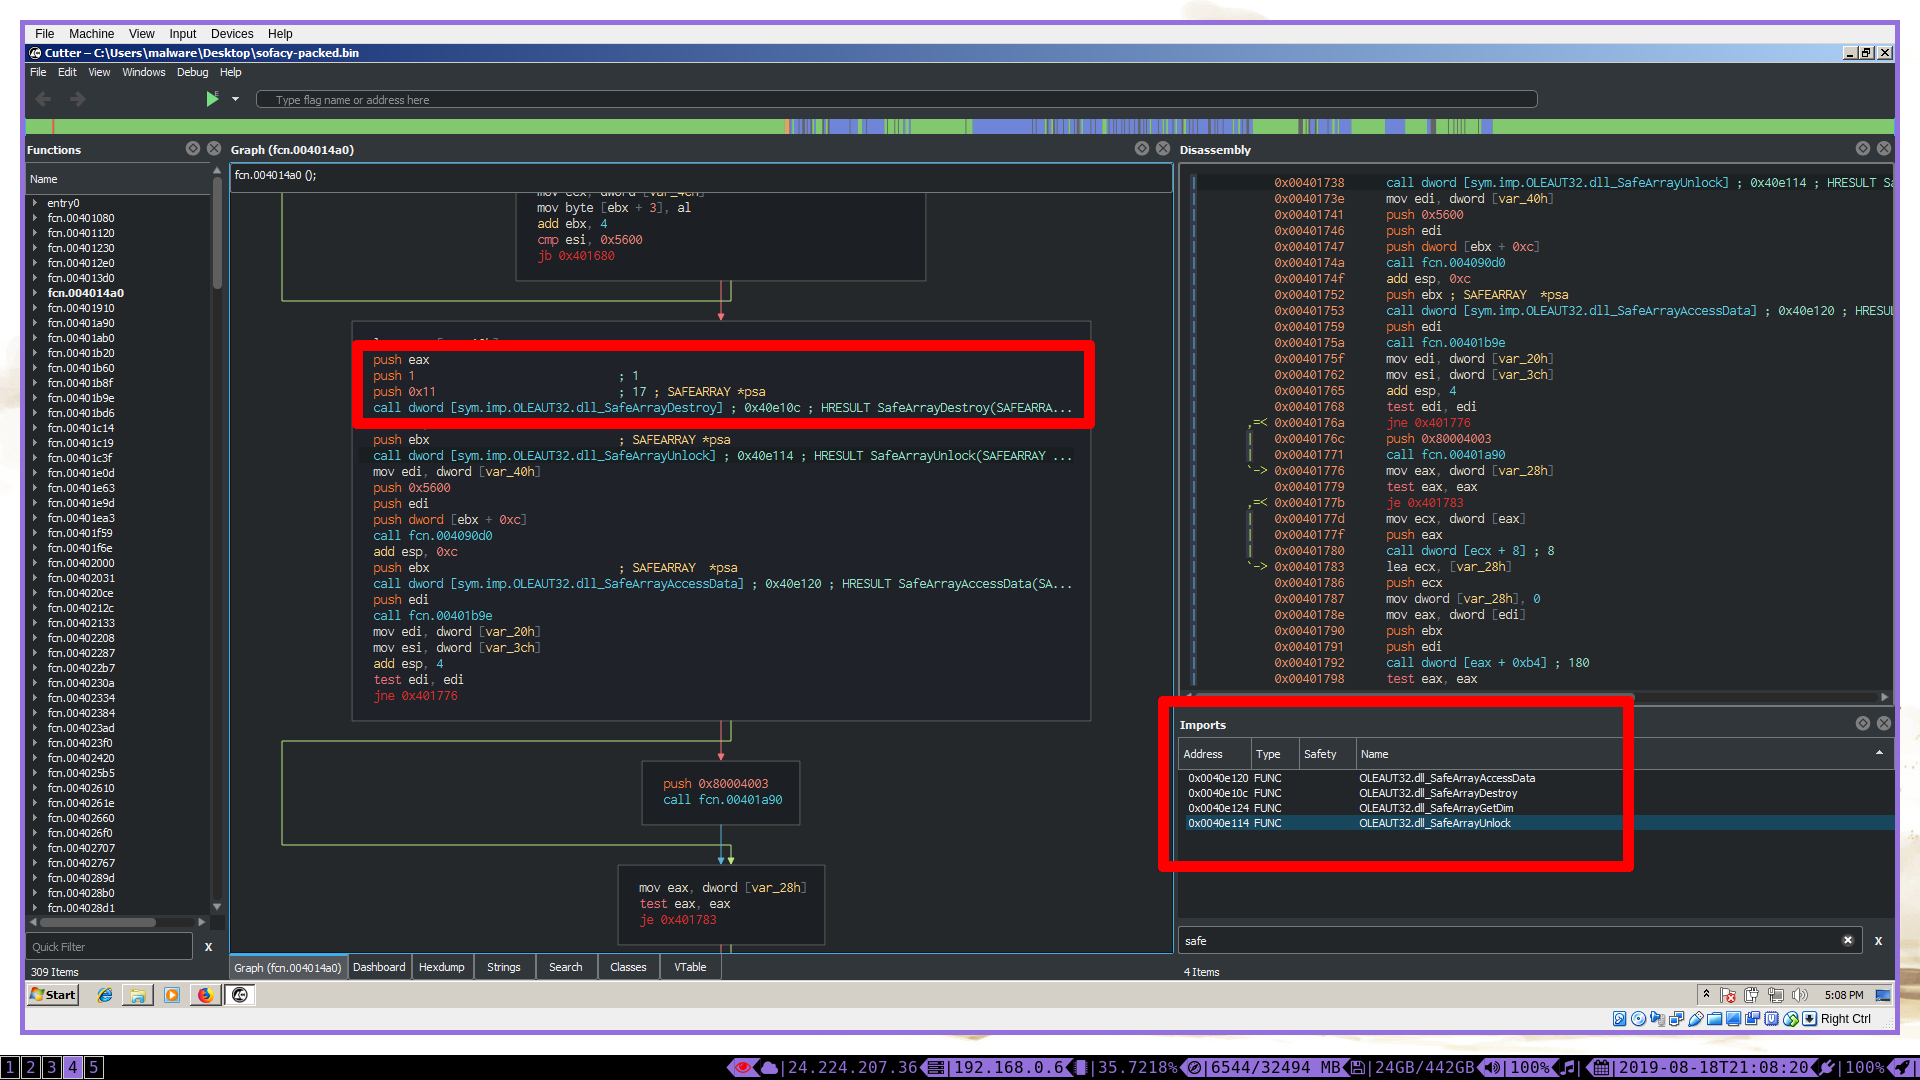
\includegraphics[scale=0.75]{cutter-navigation}
  \end{center}
\end{frame}

\begin{frame}
  \frametitle{Radare2}
  \framesubtitle{tools\_of\_the\_trade}
  \begin{center}
    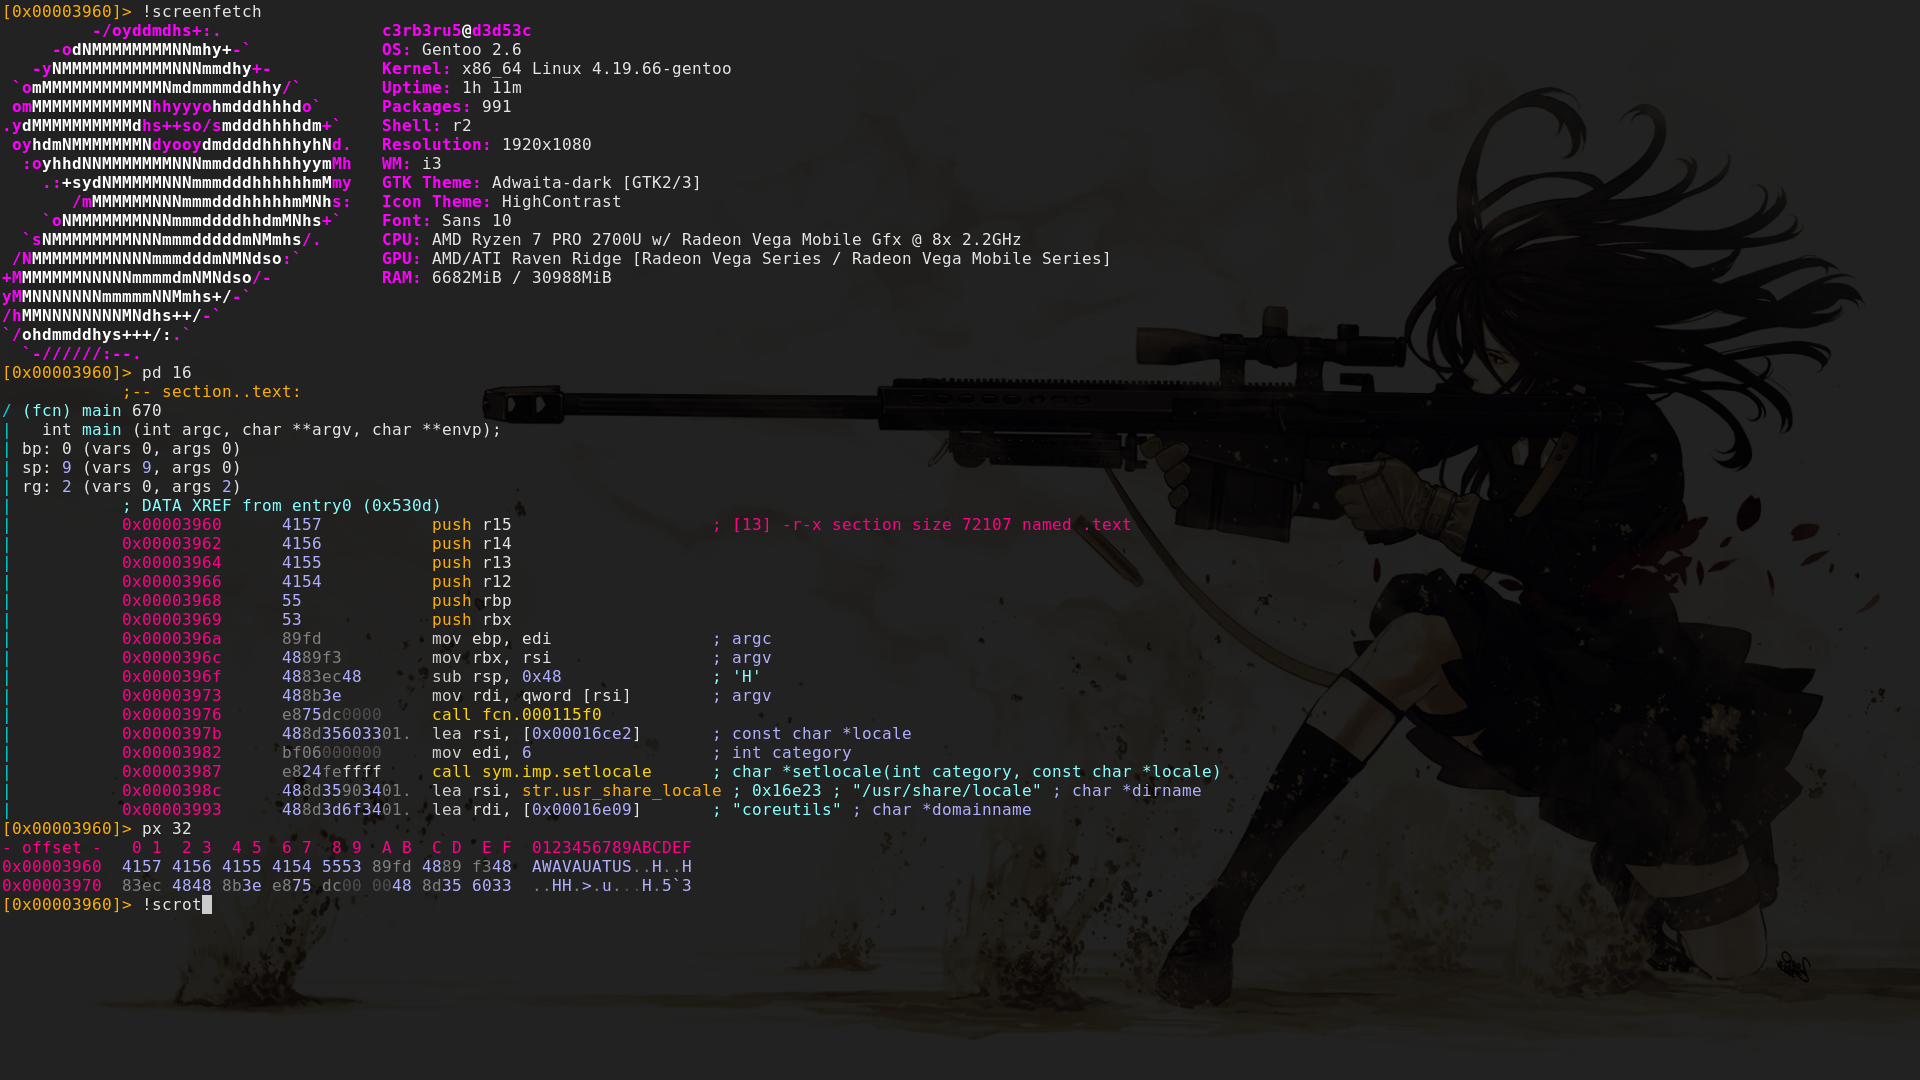
\includegraphics[scale=0.18]{radare2}
  \end{center}
\end{frame}

\begin{frame}
  \frametitle{Detect it Easy}
  \framesubtitle{tools\_of\_the\_trade}
  \begin{columns}
    \begin{column}{.2\textwidth}
      \begin{itemize}
      \item{Type}
      \item{Packer}
      \item{Linker}
      \item{Entropy}
      \end{itemize}
    \end{column}
    \hfill
    \begin{column}{.8\textwidth}
      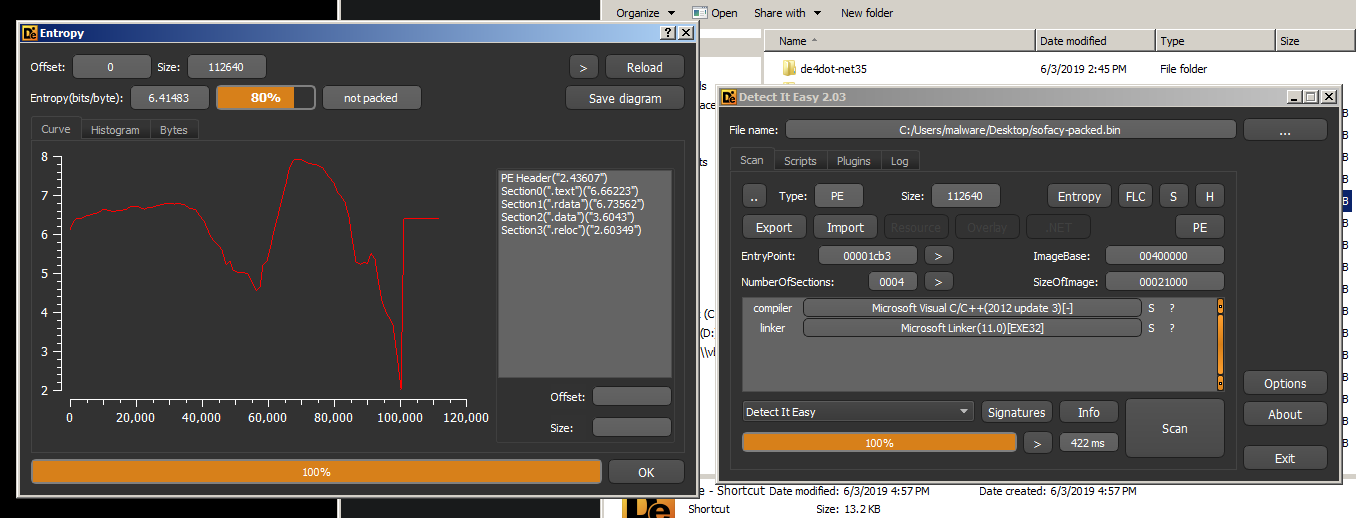
\includegraphics[scale=.98]{detect-it-easy}
    \end{column}
  \end{columns}
\end{frame}

\begin{frame}
  \frametitle{DnSpy}
  \framesubtitle{tools\_of\_the\_trade}
  \begin{columns}
    \begin{column}{.3\textwidth}
      \begin{itemize}
        \item{Code View}
        \item{Debugging}
        \item{Unpacking}
      \end{itemize}
    \end{column}
    \hfill
    \begin{column}{.7\textwidth}
      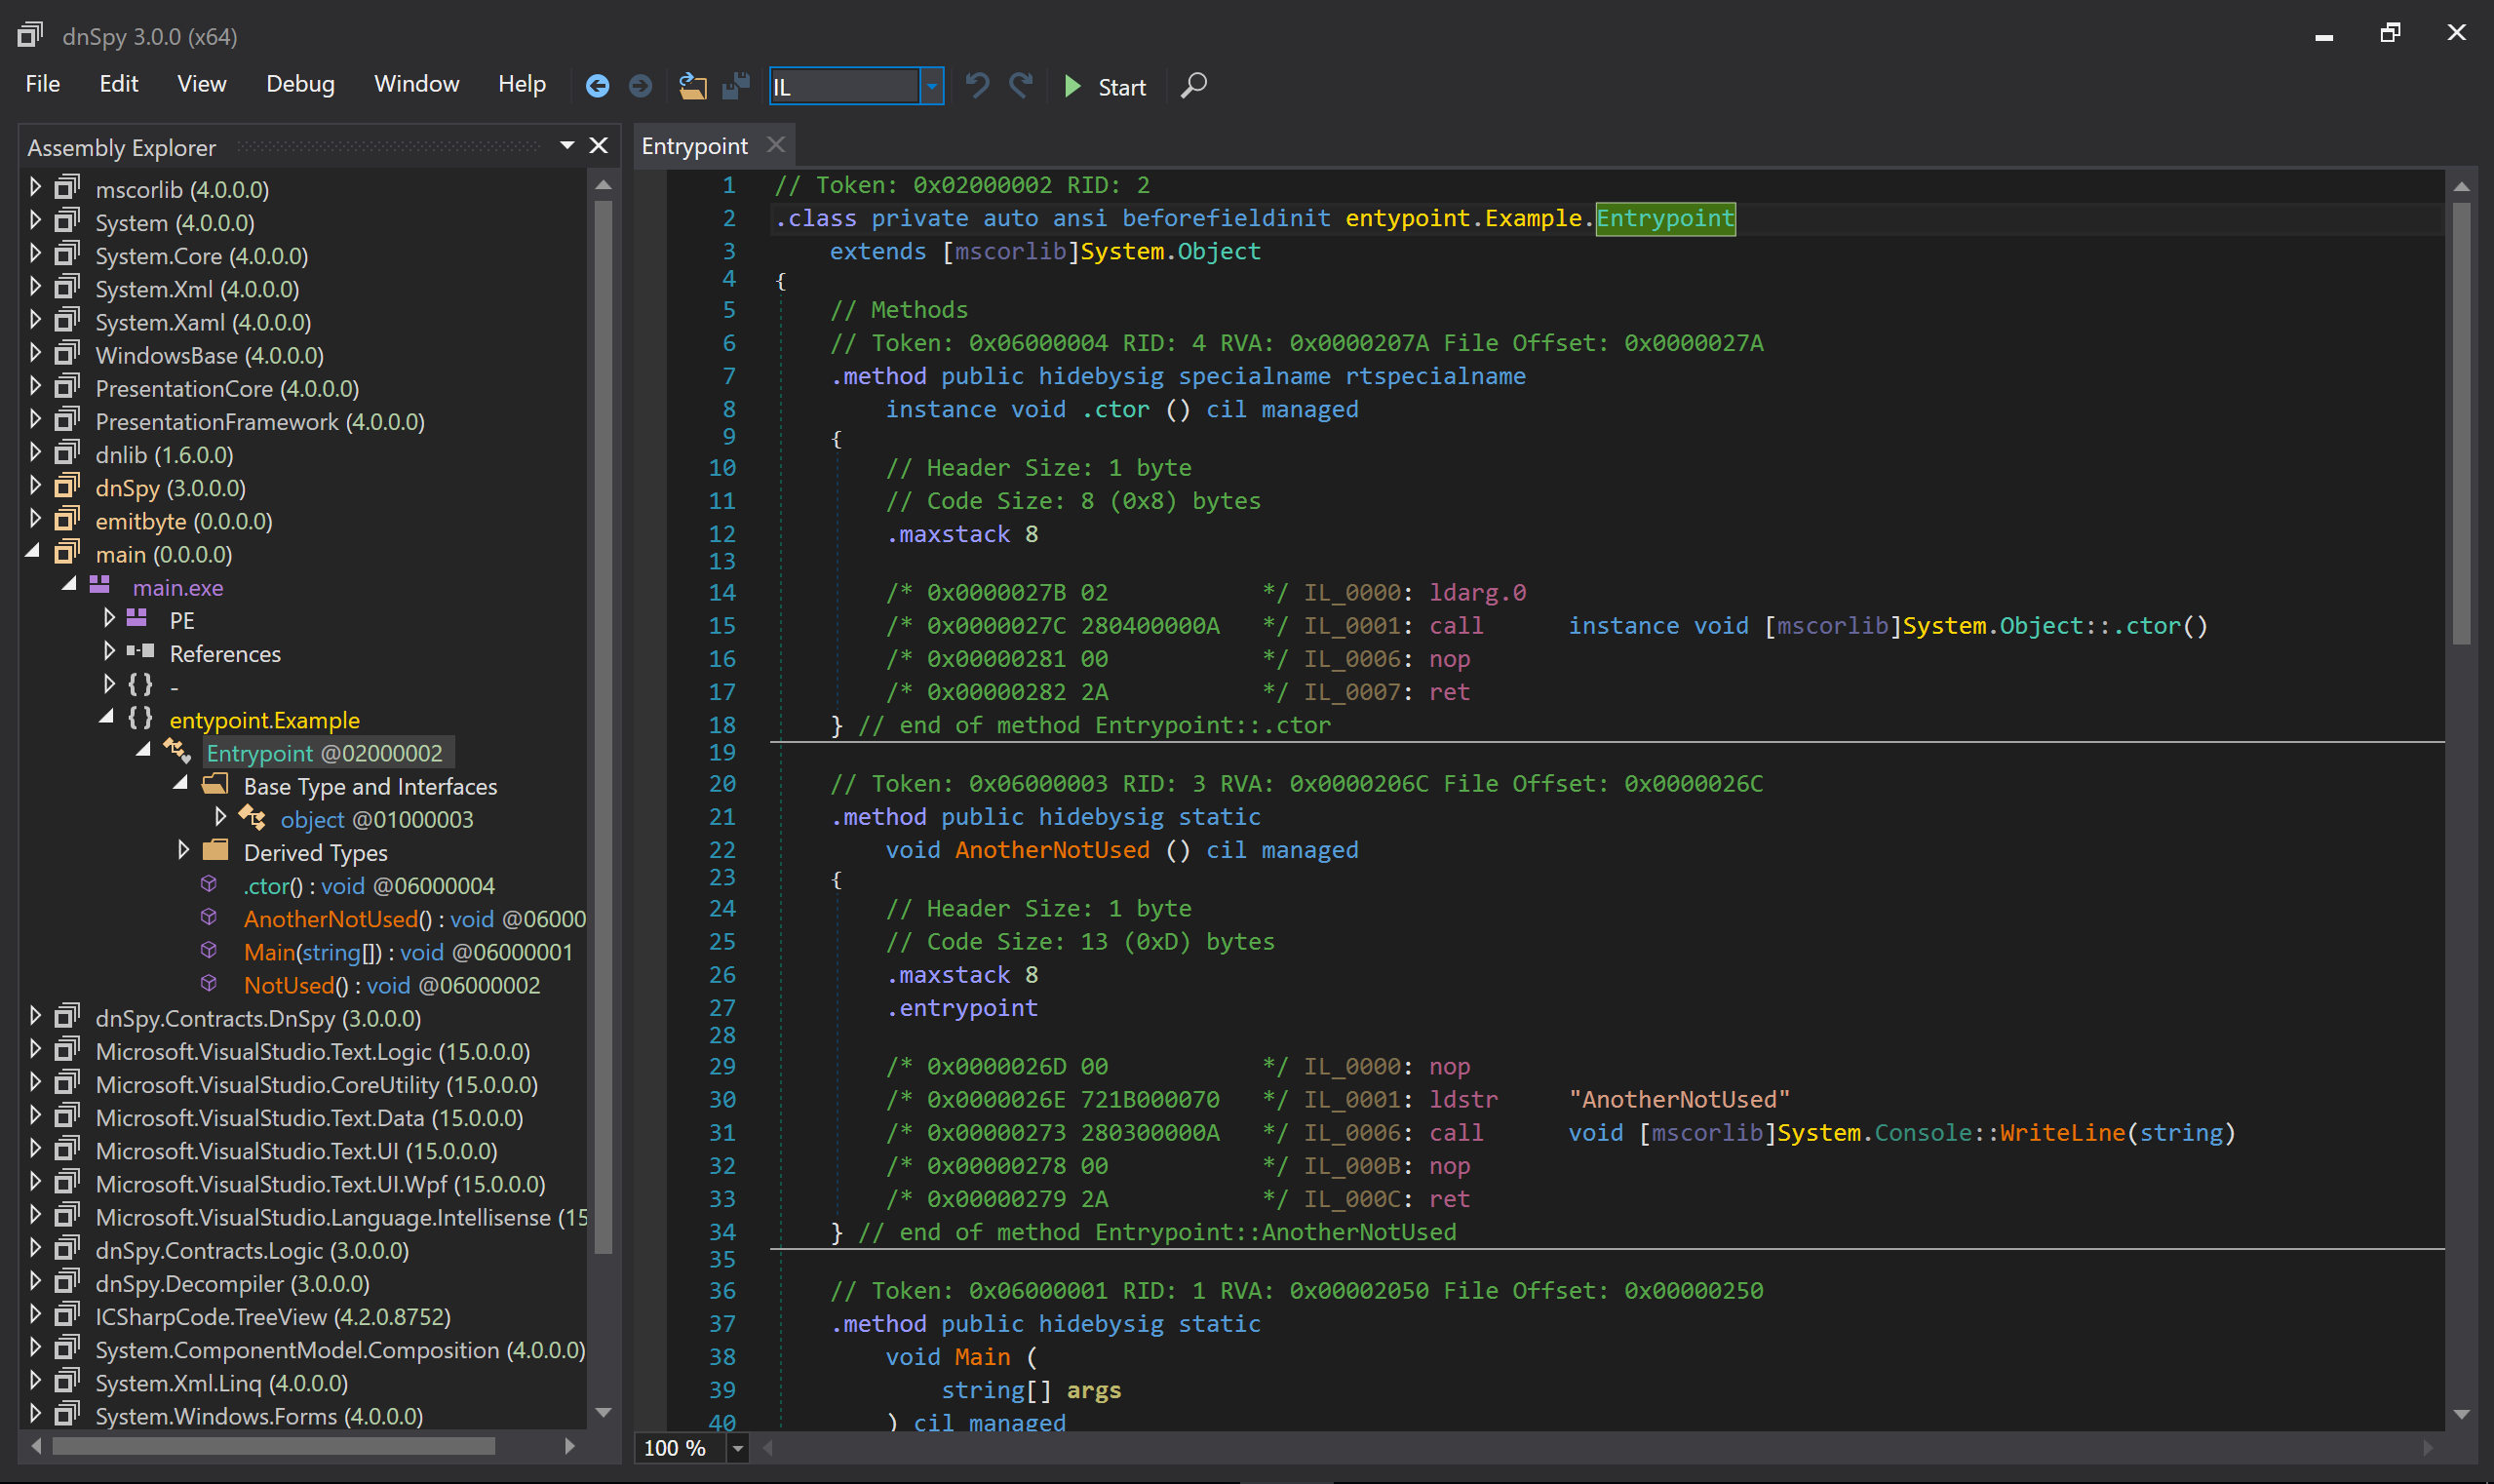
\includegraphics[scale=0.22]{dnspy}
    \end{column}
  \end{columns}
\end{frame}

\begin{frame}
  \frametitle{Useful Linux Commads}
  \framesubtitle{tools\_of\_the\_trade}
  \begin{center}
    \begin{tcolorbox}[title=terminal,colback=black]
      \begin{minipage}{0.8\textwidth}
        \textbf{\textcolor{green}{malware@work \textcolor{blue}{\~ \$}}}
        \textcolor{white}{ file sample.bin}
        \newline
        \textcolor{white}{ sample.bin: PE32 executable (GUI) Intel 80386, for MS Windows}
        \newline
        \textbf{\textcolor{green}{malware@work \textcolor{blue}{\~ \$}}}
        \textcolor{white}{ exiftool sample.bin $>$ metadata.log}
        \newline
        \textbf{\textcolor{green}{malware@work \textcolor{blue}{\~ \$}}} \textcolor{white}{ hexdump -C -n 128 sample.bin $|$ less}
        \newline
        \textbf{\textcolor{green}{malware@work \textcolor{blue}{\~ \$}}}
        \textcolor{white}{ VBoxManage list vms}
        \newline
        \textcolor{white}{"win10" \{53014b4f-4c94-49b0-9036-818b84a192c9\}\newline"win7" \{942cde2e-6a84-4edc-b98a-d7326b4662ee\}}
        \newline
        \textbf{\textcolor{green}{malware@work \textcolor{blue}{\~ \$}}}
        \textcolor{white}{ VBoxManage startvm win7}
        \newline
        \textbf{\textcolor{green}{malware@work \textcolor{blue}{\~ \$}}}
      \end{minipage}
    \end{tcolorbox}
  \end{center}
\end{frame}

\begin{frame}
  \frametitle{de4dot}
  \framesubtitle{tools\_of\_the\_trade}
  \begin{columns}
    \begin{column}{.3\textwidth}
      \begin{itemize}
      \item{Automated}
      \item{Deobfuscation}
      \item{Unpacking}
      \end{itemize}
    \end{column}
    \hfill
    \begin{column}{.7\textwidth}
      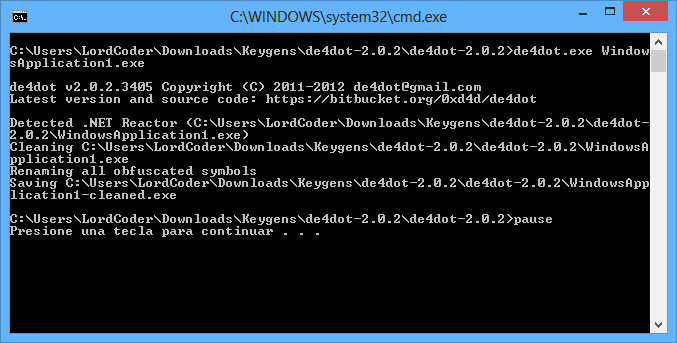
\includegraphics[scale=.55]{de4dot}
    \end{column}
  \end{columns}
\end{frame}

\begin{frame}
  \frametitle{pe-sieve}
  \framesubtitle{tools\_of\_the\_trade}
  \begin{columns}
    \begin{column}{.5\textwidth}
      \begin{itemize}
      \item{Unpacking}
      \item{Process Hollowing Extraction}
      \item{Dump Processes}
      \end{itemize}
    \end{column}
    \hfill
    \begin{column}{.5\textwidth}
      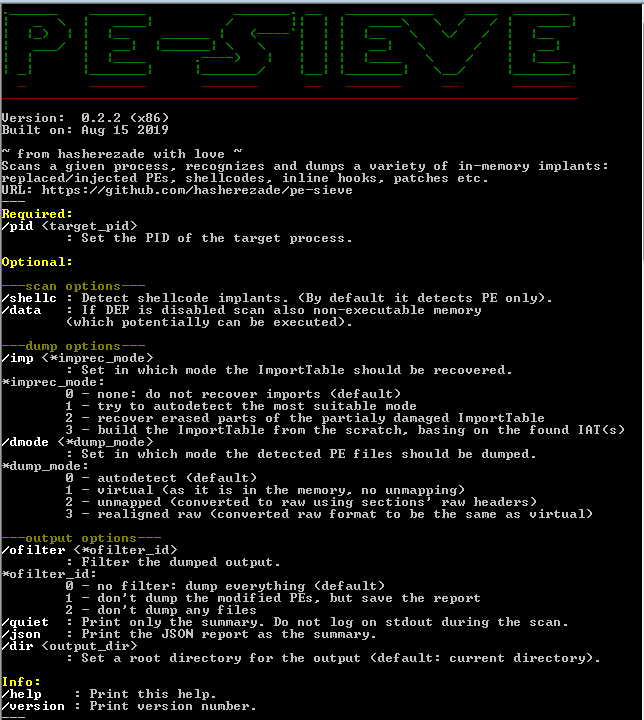
\includegraphics[scale=.28]{pe-sieve}
    \end{column}
  \end{columns}
\end{frame}

\begin{frame}
  \frametitle{Injection Techniques}
  \begin{center}
    
\includegraphics[scale=.275]{injection-meme}
  \end{center}
\end{frame}

\begin{frame}
  \frametitle{DLL Injection}
  \framesubtitle{injection\_techniques}
  \begin{columns}
    \begin{column}{.3\textwidth}
      \begin{itemize}
      \item{Get Handle to Target Process}
      \item{Allocate Memory}
      \item{Write Memory}
      \item{Execute by use of Remote Thread} 
      \end{itemize}
    \end{column}
    \hfill
    \begin{column}{.7\textwidth}
      \begin{center}
        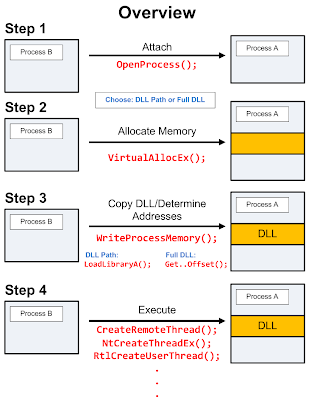
\includegraphics[scale=0.5]{dll-injection}
      \end{center}
    \end{column}
  \end{columns}
\end{frame}

\begin{frame}
  \frametitle{PE (Portable Executable) Injection}
  \framesubtitle{injection\_techniques}
  \begin{columns}
    \begin{column}{.5\textwidth}
      \begin{itemize}
      \item{Obtain Handle to Target Process}
      \item{Inject Image to Target Process}
      \item{Modify Base Address}
      \item{Modify Relocation Data}
        % table of addresses to be modified on load from unmapped to mapped
      \item{Execute your Payload}
      \end{itemize}
    \end{column}
    \hfill
    \begin{column}{.5\textwidth}
      \begin{center}
        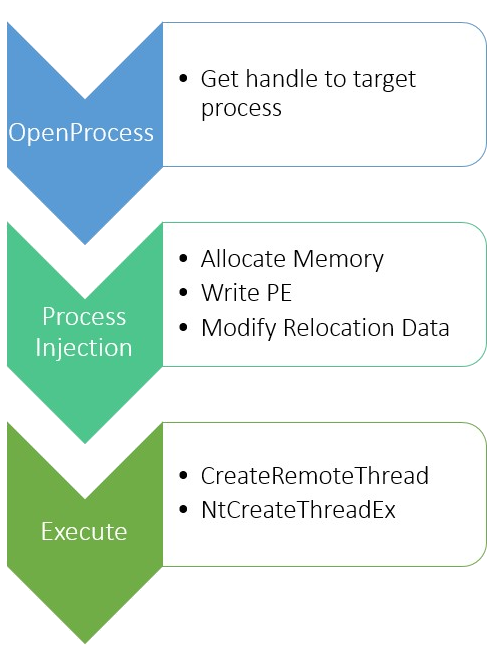
\includegraphics[scale=0.4]{pe-injection}
      \end{center}
    \end{column}
  \end{columns}
\end{frame}

\begin{frame}
  \frametitle{Atom Bombing}
  \framesubtitle{injection\_techniques}
  \begin{columns}
    \begin{column}{.4\textwidth}
      \begin{itemize}
        \item{Open Target Process}
        \item{Get Handle to Alertable Thread}
        \item{Find Code Cave}
        \item{Shellcode to Call ZwAllocateVirtualMemory and memcpy}
        \item{Call GlobalAddAtom}
        \item {Suspend Target Thread}
        \item{NtQueueApcThread}
        \item{Resume Target Thread}
      \end{itemize}
    \end{column}
    \hfill
    \begin{column}{.6\textwidth}
      \begin{center}
        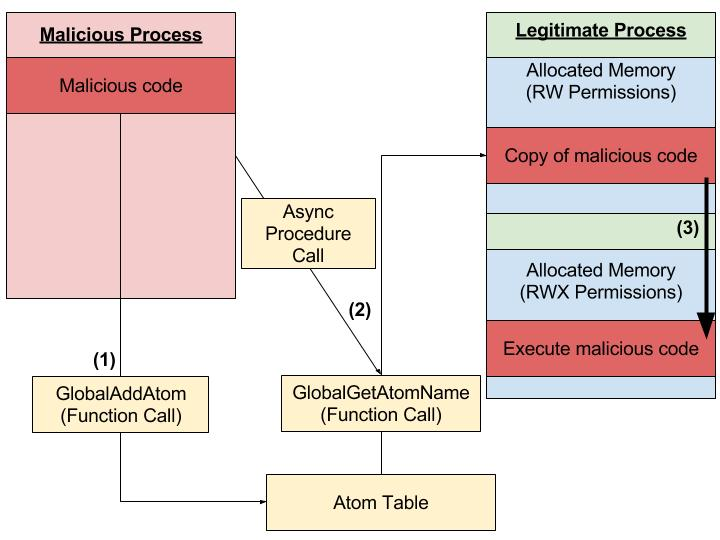
\includegraphics[scale=0.30]{atom-bombing}
      \end{center}
    \end{column}
  \end{columns}
  % An atom table is a system-defined table that stores strings and corresponding identifiers. An application places a string in an atom table and receives a 16-bit integer, called an atom, that can be used to access the string. A string that has been placed in an atom table is called an atom name.
\end{frame}

\begin{frame}
  \frametitle{Process Hollowing}
  \framesubtitle{injection\_techniques}
  \begin{columns}
    \begin{column}{.5\textwidth}
      \begin{itemize}
      \item{Create Suspended Process}
      \item{Hollow Process with NtUnmapViewOfSection}
      \item{Allocate Memory in Process}
      \item{Write Memory to Process}
      \item{Resume Thread / Process}
      \end{itemize}
    \end{column}
    \hfill
    \begin{column}{.5\textwidth}
      \begin{center}
        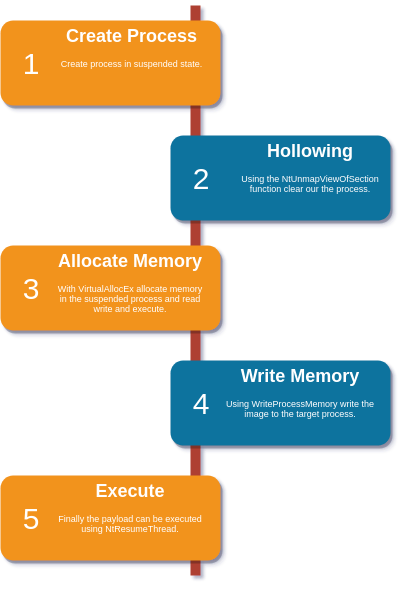
\includegraphics[scale=0.35]{process-hollowing}
      \end{center}
    \end{column}
  \end{columns}
\end{frame}

\begin{frame}
  \frametitle{Let's Try Not to Mess this Up}
  \begin{center}
    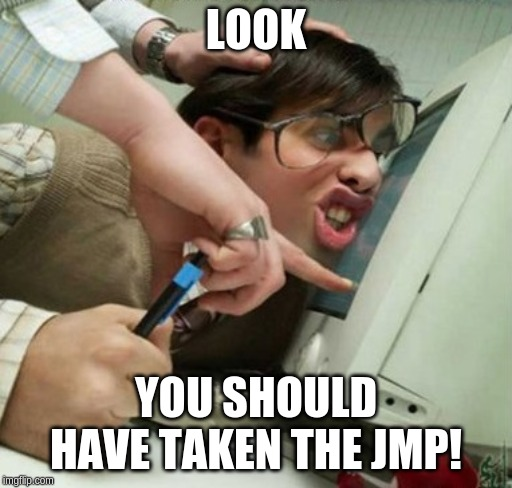
\includegraphics[width=7cm]{jmp-meme}
  \end{center}
\end{frame}

{\usebackgroundtemplate{
\includegraphics[width=\paperwidth]{malspam-background.png}}
\begin{frame}
  \frametitle{Operation Lawyer Loot}
  \framesubtitle{Initial Infection Vector}
  \begin{tabularx}{\textwidth}{ |X|X| }
    \hline
    \multicolumn{2}{|c|}{\textbf{MalSpam Email}} \\
    \hline
    \textbf{From:} & \textbf{\textcolor{red}{$<$sidney.m[at]carmellaw[.]com$>$}} \\
    \hline
    \textbf{Subject:} & Wire confirmation \\
    \hline
    \textbf{Attached:} & img-000310519000.img \\
    \hline
    \textbf{Body:} & Hello,
    \newline
    \newline
    Kindly find attached the confirmation for your reference
    \newline
    \newline
    please revert back ASAP
    \newline
    \newline
    Regards
    \newline
    \newline
    Sidney morris \\
    \hline
  \end{tabularx}
\end{frame}
}

{\usebackgroundtemplate{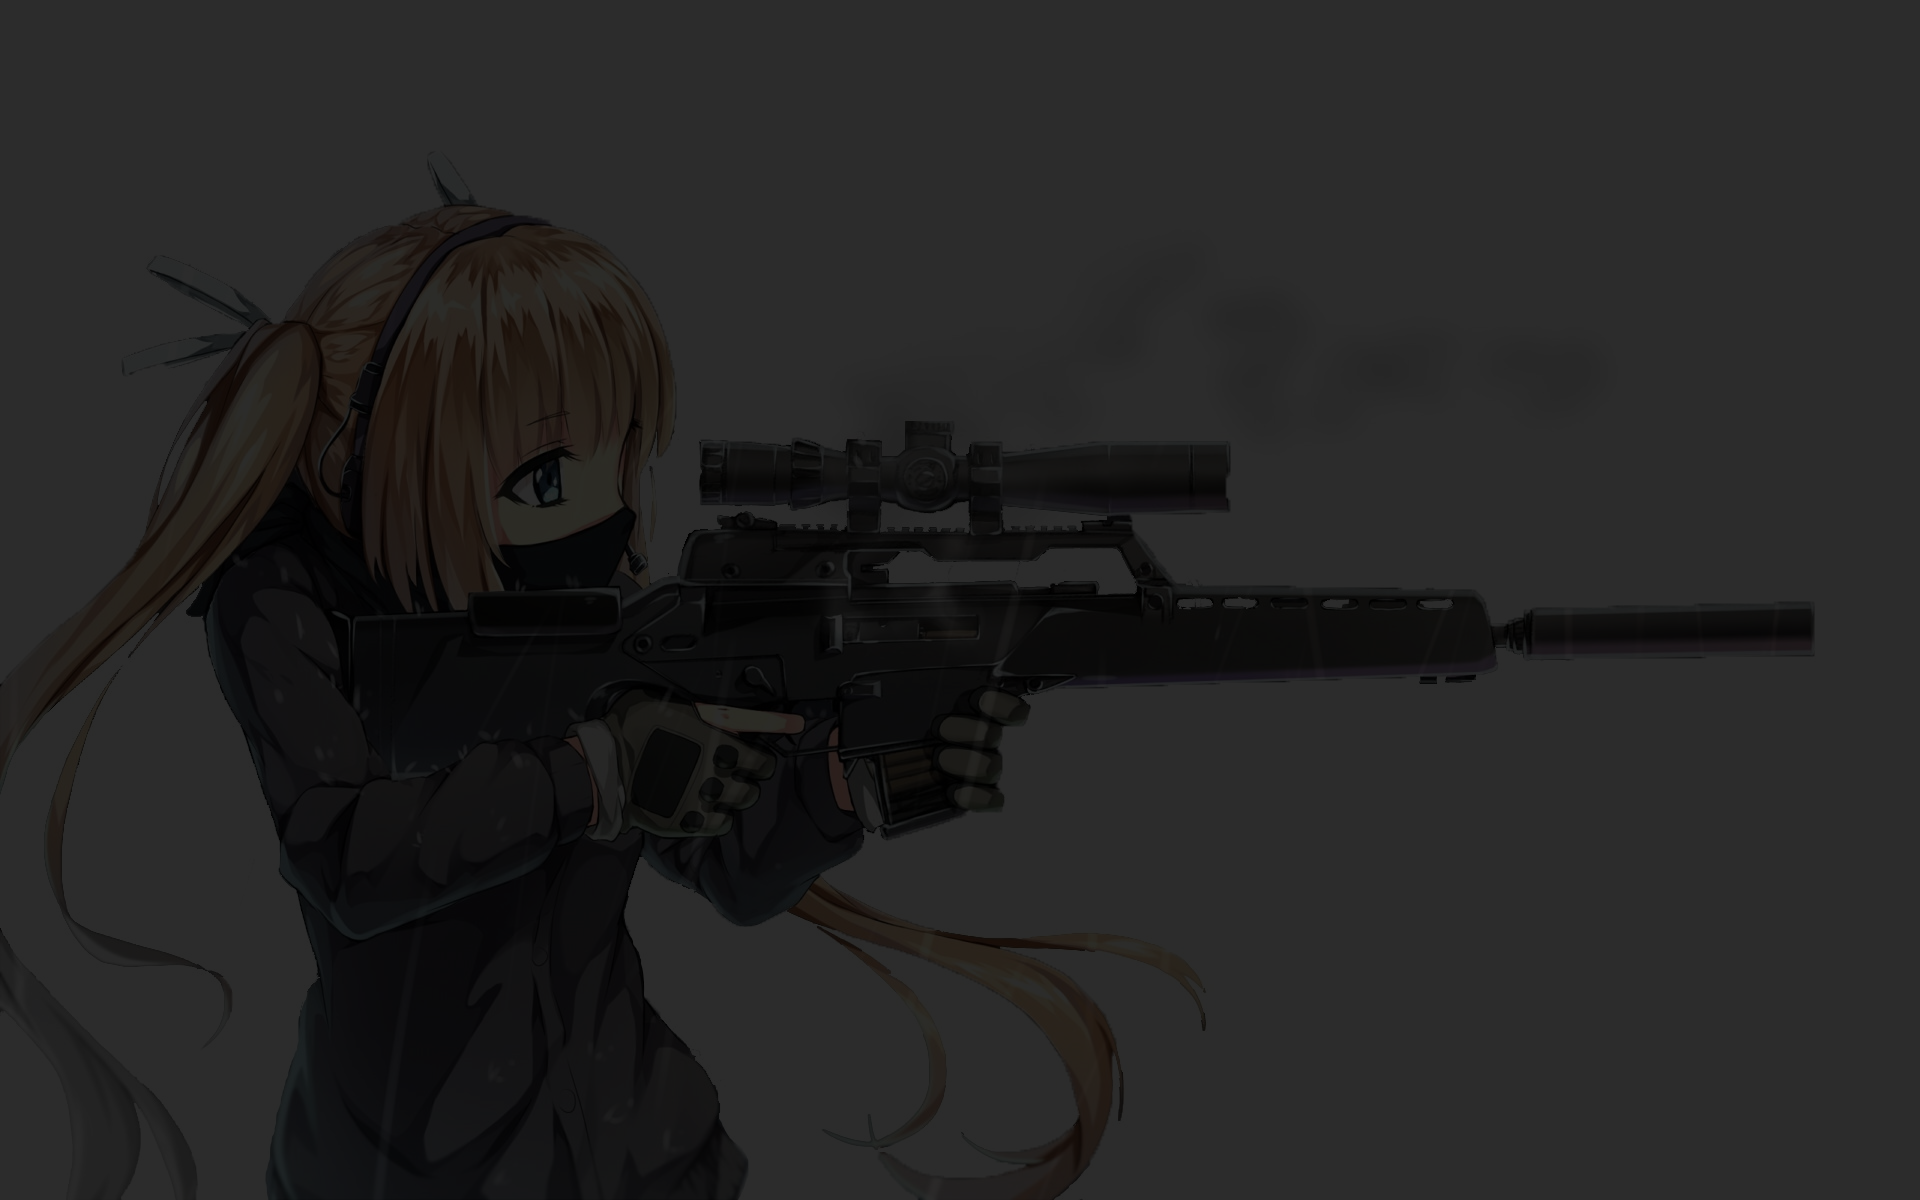
\includegraphics[width=\paperwidth]{anime-sniper-background.png}}%
\begin{frame}
  \frametitle{Operation Lawyer Loot}
  \framesubtitle{Campaign Targets}
  \begin{itemize}
    \item{Inbox Detection and Response (IDR)} Team
    \item{Lawyers}
    \item{Real Estate Agents}
    \item{Accountants}
    \item{Tax Firms}
  \end{itemize}
\end{frame}
}

{\usebackgroundtemplate{
\includegraphics[width=\paperwidth]{digital-background.jpg}}
\begin{frame}
  \frametitle{Operation Lawyer Loot}
  \framesubtitle{Extracting the Payload}
  \AddToShipoutPictureFG*{
    \makebox(810,100){
\includegraphics[width=3cm]{anime-computer-clipart}}
  }
  \begin{center}
    \begin{tcolorbox}[title=terminal,colback=black]
      \begin{minipage}{0.8\textwidth}
        \textbf{\textcolor{green}{malware@localhost \textcolor{blue}{\~ \$}}}
        \textcolor{white}{md5sum img-000310519000.img}
        \newline
        \textcolor{white}{5466c52191ddd1564b4680060dc329cb  img-000310519000.img}
        \newline
        \textbf{\textcolor{green}{malware@localhost \textcolor{blue}{\~ \$}}}
        \textcolor{white}{ file img-000310519000.img}
        \newline
        \textcolor{white}{UDF filesystem data (version 1.5) NEW\_FOLDER\_2\_}
        \newline
        \textbf{\textcolor{green}{malware@localhost \textcolor{blue}{\~ \$}}}
        \textcolor{white}{ 7z e img-000310519000.img}
        \newline
        \textbf{\textcolor{green}{malware@localhost \textcolor{blue}{\~ \$}}}
        \textcolor{white}{ file img-00031051900.exe}
        \newline
        \textcolor{white}{PE32 executable (GUI) Intel 80386 Mono/.Net assembly, for MS Windows}
        \newline
        \textbf{\textcolor{green}{malware@localhost \textcolor{blue}{\~ \$}}}
      \end{minipage}
    \end{tcolorbox}
  \end{center}
\end{frame}
}

{\usebackgroundtemplate{
\includegraphics[width=\paperwidth]{digital-background.jpg}}
\begin{frame}
  \frametitle{Operation Lawyer Loot}
  \framesubtitle{Portex Analyzer Entropy Stage 1}
  \AddToShipoutPictureFG*{
    \makebox(775,170){
\includegraphics[width=6cm]{anime-wink}}
  }
  \begin{center}
    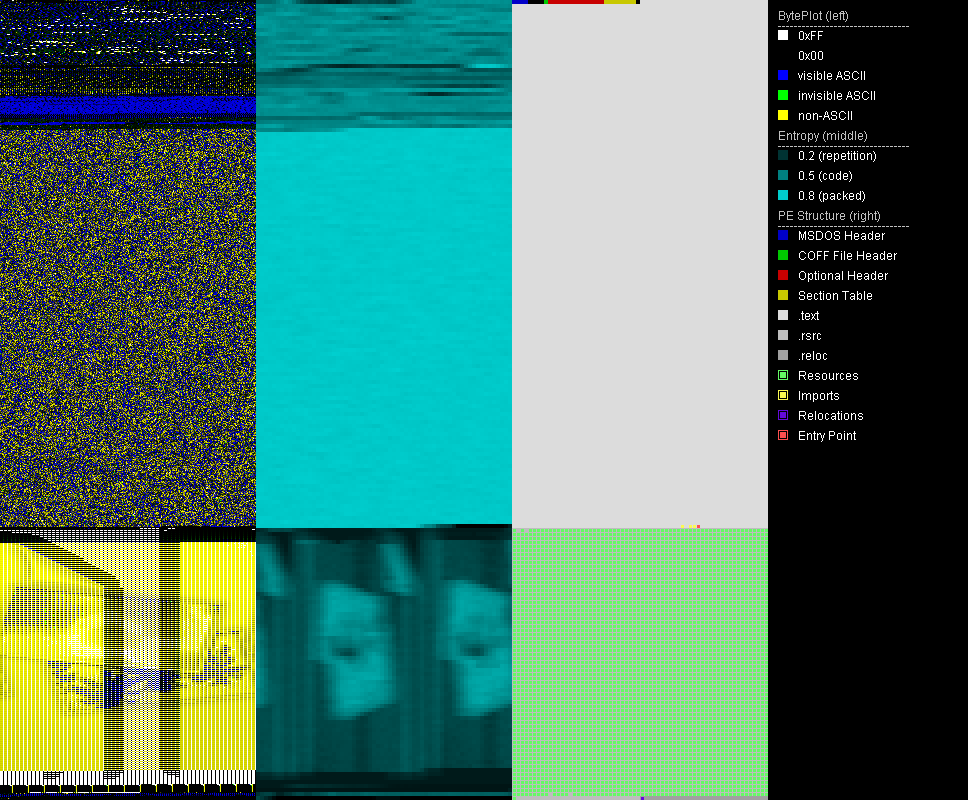
\includegraphics[width=8cm]{kpot-portex-analyzer-stage-1}
  \end{center}
\end{frame}
}

{\usebackgroundtemplate{
\includegraphics[width=\paperwidth]{digital-background.jpg}}
\begin{frame}
  \frametitle{Operation Lawyer Loot}
  \framesubtitle{Determining the Stage 1 Packer}
  \begin{columns}
    \begin{column}{.3\textwidth}
      \begin{itemize}
      \item{Packed with Smart Assembly}
      \item{Let's now try de4dot}
      \end{itemize}
    \end{column}
    \hfill
    \begin{column}{.7\textwidth}
      \begin{center}
        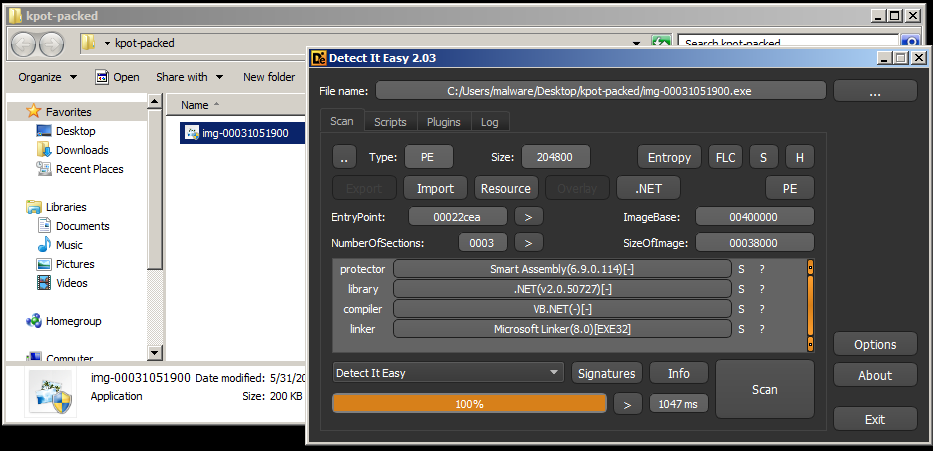
\includegraphics[scale=1.25]{kpot-unpacking-2}
      \end{center}
    \end{column}
  \end{columns}
\end{frame}
}

{\usebackgroundtemplate{
\includegraphics[width=\paperwidth]{digital-background.jpg}}
\begin{frame}
  \frametitle{Operation Lawyer Loot}
  \framesubtitle{Unpacking Stage 1}
  \begin{columns}
    \begin{column}{.3\textwidth}
      \begin{itemize}
      \item{de4dot detected smart assembly}
      \item{Let's have a look in DnSpy!}
      \end{itemize}
    \end{column}
    \hfill
    \begin{column}{.7\textwidth}
      \begin{center}
        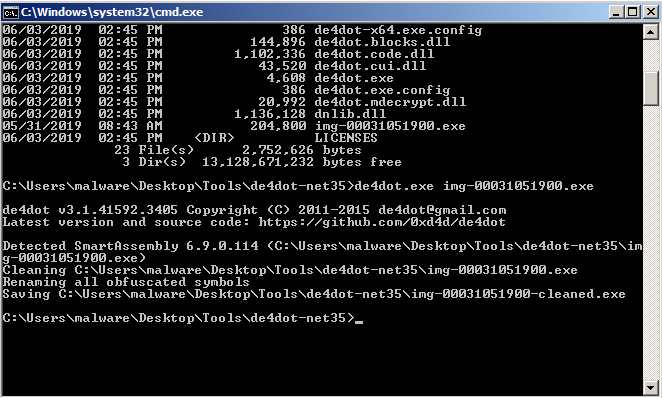
\includegraphics[scale=1.75]{kpot-unpacking-3}
      \end{center}
    \end{column}
  \end{columns}
\end{frame}
}

{\usebackgroundtemplate{
\includegraphics[width=\paperwidth]{digital-background.jpg}}
\begin{frame}
  \frametitle{Operation Lawyer Loot}
  \framesubtitle{Identifying Stage 2 Loader Packed Data}
  \begin{center}
    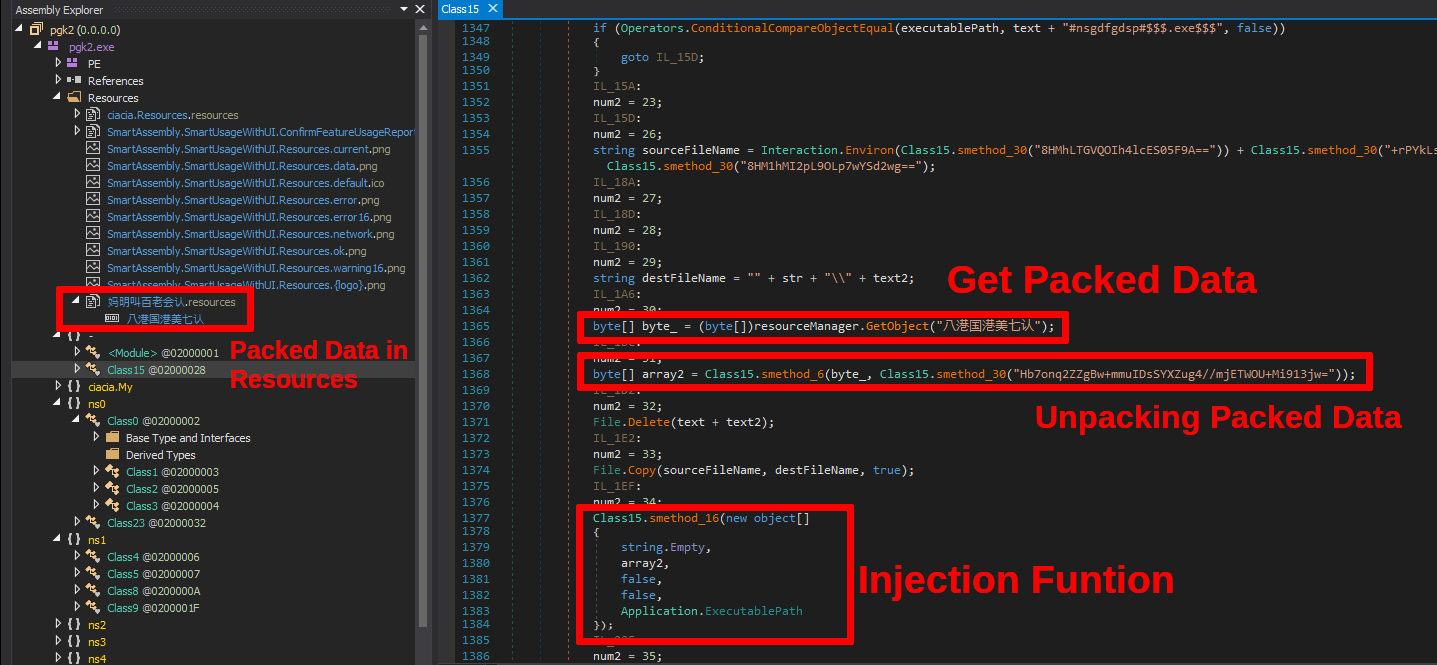
\includegraphics[width=14cm]{kpot-unpacking-4}
  \end{center}
\end{frame}
}

{\usebackgroundtemplate{
\includegraphics[width=\paperwidth]{digital-background.jpg}}
\begin{frame}
  \frametitle{Operation Lawyer Loot}
  \framesubtitle{Stage 2 Loader String Decryptor}
  \begin{columns}
    \begin{column}{.3\textwidth}
      \begin{itemize}
      \item{Uses Rijndael for string obfuscation}
      \item{We can use C\# in Visual Studio!}
      \end{itemize}
    \end{column}
    \hfill
    \begin{column}{.7\textwidth}
      \begin{center}
        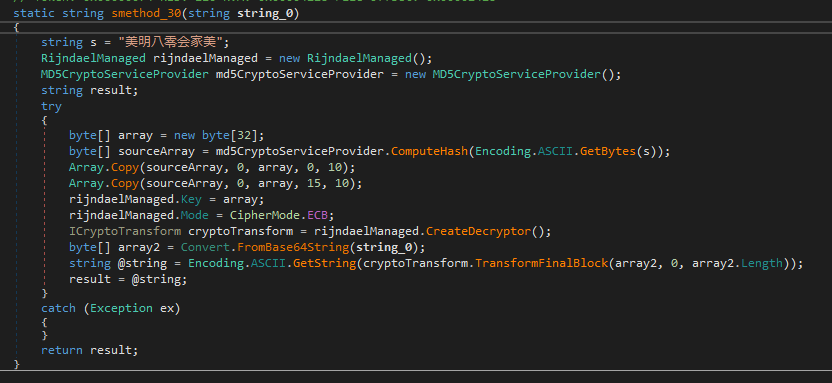
\includegraphics[scale=1.30]{kpot-unpacking-5}
      \end{center}
    \end{column}
  \end{columns}
\end{frame}
}

{\usebackgroundtemplate{
\includegraphics[width=\paperwidth]{digital-background.jpg}}
\begin{frame}[fragile]
  \frametitle{Operation Lawyer Loot}
  \framesubtitle{Stage 2 Loader Rijndael String Decryptor Key}
  \AddToShipoutPictureFG*{
    \makebox(450,105){\includegraphics[width=11cm]{anime-arms-out}}
  }
\begin{figure}
\small{
\begin{verbatim}
00000000  98 00 17 89 1f f6 7c f8  a2 0f 00 00 00 00 00 98  |......|.........|
00000010  00 17 89 1f f6 7c f8 a2  0f 00 00 00 00 00 00 00  |.....|..........|
\end{verbatim}
}
\caption{Stage 2 Loader - Rijndael Cipher Key}
\end{figure}
\end{frame}
}

{\usebackgroundtemplate{\includegraphics[width=\paperwidth]{digital-background.jpg}}
\begin{frame}
  \frametitle{Operation Lawyer Loot}
  \framesubtitle{Stage 2 Loader String Decryptor in Visual Studio}
  \begin{center}
    \includegraphics[width=13cm]{kpot-unpacking-6}
  \end{center}
\end{frame}
}

{\usebackgroundtemplate{\includegraphics[width=\paperwidth]{digital-background.jpg}}
\begin{frame}
  \frametitle{Operation Lawyer Loot}
  \framesubtitle{Stage 2 Loader Unpacking Routine Key}
  \begin{center}
    \begin{figure}
      \includegraphics[width=14cm]{stage-2-unpacking-key}
      \caption{Stage 2 Loader - Unpacking Routine Key}
    \end{figure}
  \end{center}
\end{frame}
}

{\usebackgroundtemplate{\includegraphics[width=\paperwidth]{digital-background.jpg}}
\begin{frame}
  \frametitle{Operation Lawyer Loot}
  \framesubtitle{Stage 2 Loader Decryption Routine}
  \begin{figure}
    \includegraphics[width=10cm]{stage-2-unpacking-routine}
    \caption{Stage 2 Loader - Payload Decryption Routine}
  \end{figure}
\end{frame}
}

{\usebackgroundtemplate{\includegraphics[width=\paperwidth]{digital-background.jpg}}
\begin{frame}
  \frametitle{Operation Lawyer Loot}
  \framesubtitle{Stage 2 Loader Injection Attempts}
  \begin{figure}
    \includegraphics[width=10cm]{injection-attempts}
    \caption{Stage 2 Loader - Injection Attempts}
  \end{figure}
\end{frame}
}


{\usebackgroundtemplate{\includegraphics[width=\paperwidth]{digital-background.jpg}}
\begin{frame}
  \frametitle{Operation Lawyer Loot}
  \framesubtitle{Stage 2 Loader Injection Method}
  \begin{center}
    \begin{figure}
      \includegraphics[scale=1.28]{kpot-unpacking-8}
      \caption{Unpacking KPot - API Function Name Encryption}
    \end{figure}
  \end{center}
\end{frame}
}

{\usebackgroundtemplate{\includegraphics[width=\paperwidth]{digital-background.jpg}}
\begin{frame}
  \frametitle{Operation Lawyer Loot}
  \framesubtitle{Stage 2 Loader Injection API Function Name Decryption}
  \begin{center}
    \begin{figure}
      \includegraphics[width=12cm]{kpot-unpacking-9}
      \caption{Unpacking KPot - Decrypt Injection API Function Names}
    \end{figure}
  \end{center}
\end{frame}
}

{\usebackgroundtemplate{\includegraphics[width=\paperwidth]{digital-background.jpg}}
\begin{frame}[fragile]
  \frametitle{Operation Lawyer Loot}
  \framesubtitle{Stage 2 Loader RFC-2898 / Rijndael
    String Decryptor Key}
  \AddToShipoutPictureFG*{
    \makebox(125,150){\includegraphics[width=6cm]{anime-peace}}
  }
\begin{figure}
\small{
\begin{verbatim}
00000000  ee 77 8a 97 5f 56 f8 56  fa 18 82 54 d8 f3 a6 91  |.w.._V.V...T....|
00000010  d0 ef 76 2a 21 b3 ab 1c  eb 8d 61 04 ec c7 50 96  |..v*!.....a...P.|
\end{verbatim}
}
\caption{Stage 2 Loader - RFC-2898 / Rijndael String Decryption Key}
\end{figure}
\end{frame}
}



{\usebackgroundtemplate{\includegraphics[width=\paperwidth]{digital-background.jpg}}
\begin{frame}
  \frametitle{Operation Lawyer Loot}
  \framesubtitle{Stage 2 Loader Injection API Function Name Decryption}
  \begin{center}
    \begin{figure}
      \includegraphics[width=14cm]{kpot-unpacking-10}
      \caption{Unpacking KPot - Process Hollowing Functions}
    \end{figure}
  \end{center}
\end{frame}
}

{\usebackgroundtemplate{\includegraphics[width=\paperwidth]{digital-background.jpg}}
\begin{frame}
  \frametitle{Operation Lawyer Loot}
  \framesubtitle{Stage 2 Loader Unpacking Process Hollowing
    with pe-sieve}
  \begin{center}
    \includegraphics[width=14cm]{kpot-unpacking-11}
  \end{center}
\end{frame}
}

{\usebackgroundtemplate{\includegraphics[width=\paperwidth]{digital-background.jpg}}
\begin{frame}
  \frametitle{Operation Lawyer Loot}
  \framesubtitle{KPot v2.0 Strings}
  \begin{center}
    \includegraphics[scale=0.95]{kpot-unpacking-12}
  \end{center}
\end{frame}
}

{\usebackgroundtemplate{\includegraphics[width=\paperwidth]{digital-background.jpg}}
\begin{frame}
  \frametitle{Operation Lawyer Loot}
  \framesubtitle{KPot v2.0 Final Payload in C++}
  \begin{center}
    \includegraphics[width=10cm]{kpot-unpacking-13}
  \end{center}
\end{frame}
}

{\usebackgroundtemplate{\includegraphics[width=\paperwidth]{digital-background.jpg}}
\begin{frame}
  \frametitle{Operation Lawyer Loot}
  \framesubtitle{KPot v2.0 - Final Payload Portex Analyzer Entropy}
  \begin{center}
    \includegraphics[width=10cm]{unpacked-portex-analyzer}
  \end{center}
\end{frame}
}

{\usebackgroundtemplate{\includegraphics[width=\paperwidth]{digital-background.jpg}}
\begin{frame}
  \frametitle{Are we done?}
  \begin{center}
    \includegraphics[width=10cm]{frustrated-meme}
  \end{center}
\end{frame}
}

{\usebackgroundtemplate{\includegraphics[width=\paperwidth]{digital-background.jpg}}
\begin{frame}
  \frametitle{Operation Lawyer Loot}
  \framesubtitle{KPot v2.0 - Initialization}
  \begin{figure}
    \includegraphics[width=8cm]{kpot-entry0}
    \caption{KPot v2.0 - Initialization}
  \end{figure}
\end{frame}
}

{\usebackgroundtemplate{\includegraphics[width=\paperwidth]{digital-background.jpg}}
\begin{frame}
  \frametitle{Operation Lawyer Loot}
  \framesubtitle{KPot v2.0 - Disabling ASLR}
  \AddToShipoutPictureFG*{
    \makebox(75,140){\includegraphics[width=4cm]{anime-headphones}}
  }
  \begin{center}
    \includegraphics[width=10cm]{kpot-disable-aslr}
  \end{center}
\end{frame}
}

{\usebackgroundtemplate{\includegraphics[width=\paperwidth]{digital-background.jpg}}
\begin{frame}
  \frametitle{Operation Lawyer Loot}
  \framesubtitle{KPot v2.0 - Dynamically Resolving APIs}
  \begin{figure}
    \includegraphics[width=14cm]{kpot-resolve-apis-debug}
    \caption{KPot v2.0 - Resolve APIs Dynamically}
  \end{figure}
\end{frame}
}

{\usebackgroundtemplate{\includegraphics[width=\paperwidth]{digital-background.jpg}}
\begin{frame}
  \begin{figure}
    \frametitle{Operation Lawyer Loot}
    \framesubtitle{KPot v2.0 - Sylica Resolve APIs}
    \begin{figure}
      \includegraphics[width=12cm]{kpot-resolve-apis-sylica}
      \caption{KPot v2.0 - Sylica Resolve APIs}
    \end{figure}
  \end{figure}
\end{frame}
}

{\usebackgroundtemplate{\includegraphics[width=\paperwidth]{digital-background.jpg}}
\begin{frame}
  \frametitle{Operation Lawyer Loot}
  \framesubtitle{KPot v2.0 - Scripting / Programming}
  \begin{center}
    \includegraphics[width=8cm]{anime-programming}
  \end{center}
\end{frame}
}

{\usebackgroundtemplate{\includegraphics[width=\paperwidth]{digital-background.jpg}}
\begin{frame}
  \frametitle{Operation Lawyer Loot}
  \framesubtitle{KPot v2.0 - CnC Initialization}
  \begin{figure}
    \includegraphics[width=10cm]{kpot-cnc-init}
    \caption{KPot v2.0 - CnC Initialization}
  \end{figure}
\end{frame}
}

{\usebackgroundtemplate{\includegraphics[width=\paperwidth]{digital-background.jpg}}
\begin{frame}
  \frametitle{Operation Lawyer Loot}
  \framesubtitle{KPot v2.0 - CnC COM Initialization}
  \begin{figure}
    \includegraphics[width=10cm]{kpot-cnc-init-com}
    \caption{KPot v2.0 - CnC COM Initialization}
  \end{figure}
\end{frame}
}

{\usebackgroundtemplate{\includegraphics[width=\paperwidth]{digital-background.jpg}}
\begin{frame}
  \frametitle{Operation Lawyer Loot}
  \framesubtitle{KPot v2.0 - CnC Server Initialization}
  \AddToShipoutPictureFG*{
    \makebox(150,240){\includegraphics[width=5cm]{anime-upside-down}}
  }
  \begin{figure}
    \includegraphics[width=7cm]{kpot-cnc-init-server}
    \caption{KPot v2.0 - CnC Server Initialization}
  \end{figure}
\end{frame}
}

{\usebackgroundtemplate{\includegraphics[width=\paperwidth]{digital-background.jpg}}
\begin{frame}
  \frametitle{Operation Lawyer Loot}
  \framesubtitle{KPot v2.0 - CnC Checkin}
  \begin{figure}
    \includegraphics[width=9cm]{kpot-cnc-checkin-routine}
    \caption{KPot v2.0 - Checkin Routine}
  \end{figure}
\end{frame}
}

{\usebackgroundtemplate{\includegraphics[width=\paperwidth]{digital-background.jpg}}
\begin{frame}
  \frametitle{Operation Lawyer Loot}
  \framesubtitle{KPot v2.0 - CnC Headers / URI Setup}
  \AddToShipoutPictureFG*{
    \makebox(50,120){\includegraphics[width=4cm]{anime-fairy}}
  }
  \begin{center}
    \includegraphics[width=11cm]{kpot-cnc-checkin-routine-uri-setup}
  \end{center}
\end{frame}
}

{\usebackgroundtemplate{\includegraphics[width=\paperwidth]{digital-background.jpg}}
\begin{frame}
  \frametitle{Operation Lawyer Loot}
  \framesubtitle{KPot v2.0 - CnC Checkin Attempts}
  \AddToShipoutPictureFG*{
    \makebox(810,165){\includegraphics[width=4cm]{anime-cat}}
  }
  \begin{center}
    \includegraphics[width=10cm]{kpot-cnc-checkin-attempts}
  \end{center}
\end{frame}
}

{\usebackgroundtemplate{\includegraphics[width=\paperwidth]{digital-background.jpg}}
\begin{frame}[fragile]
  \frametitle{Operation Lawyer Loot}
  \framesubtitle{KPot v2.0 - CnC Checkin HTTP Request}
  \AddToShipoutPictureFG*{
    \makebox(785,165){\includegraphics[width=4cm]{anime-music}}
  }
\begin{figure}
\small{
\begin{verbatim}
GET /BOH9KGa4jvUsU4jL/gate[.]php HTTP/1.1
Content-Type: application/x-www-form-urlencoded
Host: benten09[.]futbol
Connection: Keep-Alive
\end{verbatim}
}
\caption{KPot v2.0 - CnC Checkin HTTP GET Request}
\end{figure}
\end{frame}
}

{\usebackgroundtemplate{\includegraphics[width=\paperwidth]{digital-background.jpg}}
\begin{frame}[fragile]
  \frametitle{Operation Lawyer Loot}
  \framesubtitle{KPot v2.0 - CnC Checkin HTTP Response}
\begin{figure}
\footnotesize{
\begin{verbatim}
HTTP/1.1 200 OK
Server: nginx/1.14.1
Date: Wed, 10 Jul 2019 17:27:40 GMT
Content-Type: text/html; charset=UTF-8
Transfer-Encoding: chunked
Connection: close
X-Powered-By: PHP/7.1.29

enhFA1kHQHsAaWUDW3xQARQWMHckfzwHbgdlBVhjWAhlf0McWmkuDnQUHX8nEj5ROzkQUxxXLhV2ChVwKAgz
bxRjWl4HUV1gHywsRkYSPncZCDZwLWQuFRQ5JEIOLBVRbhYrdTp3Mwh0CgttWhI+dxkINnAtZC4VAGhmBjUS
JXUHADl/N2kVL0IzIF0aEhVIPxYrdTp3Mwh0CgttQGMVSD9lK20vZDAIcx0GbTVoFEMuOwRAB1AYJlR9CHYP
PgpEJDkrbS9kMAhzHQZtNX0+bwwbNXAqcyMVbmlhAjUSJXUHADl/N2kuFXUdGHsnAD5vFBYwdyR/PAduBw==
\end{verbatim}
}
\caption{KPot v2.0 - CnC Checkin HTTP Response}
\end{figure}
\end{frame}
}

{\usebackgroundtemplate{\includegraphics[width=\paperwidth]{digital-background.jpg}}
\begin{frame}
  \frametitle{Operation Lawyer Loot}
  \framesubtitle{KPot v2.0 - CnC Checkin Base64 Decoding}
  \AddToShipoutPictureFG*{
    \makebox(95,165){\includegraphics[width=4cm]{anime-cold}}
  }
  \begin{figure}
    \includegraphics[width=8cm]{kpot-cnc-checkin-decoding}
    \caption{KPot v2.0 - CnC Checkin Base64 Decoding}
  \end{figure}
\end{frame}
}

{\usebackgroundtemplate{\includegraphics[width=\paperwidth]{digital-background.jpg}}
\begin{frame}[fragile]
  \frametitle{Operation Lawyer Loot}
  \framesubtitle{KPot v2.0 - CnC Checkin Response Base64 Decoded}
\begin{figure}
\footnotesize{
\begin{verbatim}
00000000  7a 78 45 03 59 07 40 7b  00 69 65 03 5b 7c 50 01  |zxE.Y.@{.ie.[|P.|
00000010  14 16 30 77 24 7f 3c 07  6e 07 65 05 58 63 58 08  |..0w$.<.n.e.XcX.|
00000020  65 7f 43 1c 5a 69 2e 0e  74 14 1d 7f 27 12 3e 51  |e.C.Zi..t...'.>Q|
00000030  3b 39 10 53 1c 57 2e 15  76 0a 15 70 28 08 33 6f  |;9.S.W..v..p(.3o|
00000040  14 63 5a 5e 07 51 5d 60  1f 2c 2c 46 46 12 3e 77  |.cZ^.Q]`.,,FF.>w|
00000050  19 08 36 70 2d 64 2e 15  14 39 24 42 0e 2c 15 51  |..6p-d...9$B.,.Q|
00000060  6e 16 2b 75 3a 77 33 08  74 0a 0b 6d 5a 12 3e 77  |n.+u:w3.t..mZ.>w|
00000070  19 08 36 70 2d 64 2e 15  00 68 66 06 35 12 25 75  |..6p-d...hf.5.%u|
00000080  07 00 39 7f 37 69 15 2f  42 33 20 5d 1a 12 15 48  |..9.7i./B3 ]...H|
00000090  3f 16 2b 75 3a 77 33 08  74 0a 0b 6d 40 63 15 48  |?.+u:w3.t..m@c.H|
000000a0  3f 65 2b 6d 2f 64 30 08  73 1d 06 6d 35 68 14 43  |?e+m/d0.s..m5h.C|
000000b0  2e 3b 04 40 07 50 18 26  54 7d 08 76 0f 3e 0a 44  |.;.@.P.&T}.v.>.D|
000000c0  24 39 2b 6d 2f 64 30 08  73 1d 06 6d 35 7d 3e 6f  |$9+m/d0.s..m5}>o|
000000d0  0c 1b 35 70 2a 73 23 15  6e 69 61 02 35 12 25 75  |..5p*s#.nia.5.%u|
000000e0  07 00 39 7f 37 69 2e 15  75 1d 18 7b 27 00 3e 6f  |..9.7i..u..{'.>o|
000000f0  14 16 30 77 24 7f 3c 07  6e 07                    |..0w$.<.n.      |
\end{verbatim}
}
\caption{KPot v2.0 - CnC Checkin Base64 Decoded}
\end{figure}
\end{frame}
}

{\usebackgroundtemplate{\includegraphics[width=\paperwidth]{digital-background.jpg}}
\begin{frame}[fragile]
  \frametitle{Operation Lawyer Loot}
  \framesubtitle{KPot v2.0 - Decoded and XOR Decrypted CnC
    Payload}
  \AddToShipoutPictureFG*{
    \makebox(80,150){\includegraphics[width=6cm]{anime-suprise}}
  }
\begin{figure}
\scriptsize{
\begin{verbatim}
111111111111111__DELIMM__[victim_public_ip_address]__DELIMM__appdata__GRABBER__*.log,*.txt,
__GRABBER__%appdata%__GRABBER__0__GRABBER__1024__DELIMM__desktop_txt__GRABBER__*.txt,
__GRABBER__%userprofile%\Desktop__GRABBER__0__GRABBER__150__DELIMM____DELIMM____DELIMM__
\end{verbatim}
}
\caption{KPot v2.0 - CnC Decoded and Decrypted Response}
\end{figure}
\end{frame}
}

{\usebackgroundtemplate{\includegraphics[width=\paperwidth]{digital-background.jpg}}
\begin{frame}
  \frametitle{Operation Lawyer Loot}
  \framesubtitle{KPot v2.0 - CnC Checkin Routine Language Check}
  \AddToShipoutPictureFG*{
    \makebox(815,126){\includegraphics[width=4cm]{anime-worried}}
  }
  \begin{figure}
    \includegraphics[width=11cm]{kpot-cnc-checkin-lang-check}
    \caption{KPot v2.0 - CnC Checkin Routine Language Check}
  \end{figure}
\end{frame}
}

{\usebackgroundtemplate{\includegraphics[width=\paperwidth]{digital-background.jpg}}
\begin{frame}
  \frametitle{Operation Lawyer Loot}
  \framesubtitle{KPot v2.0 - Language List}
  \AddToShipoutPictureFG*{
    \makebox(675,210){\includegraphics[width=9cm]{anime-point-left}}
  }
  \begin{itemize}
  \item{LANG\_RUSSIAN}
  \item{LANG\_ARMENIAN}
  \item{LANG\_AZERI}
  \item{LANG\_SUBLANG\_AZERI\_LATIN}
  \item{LANG\_GEORGIAN}
  \item{LANG\_TAJIK}
  \item{LANG\_CROATIAN}
  \item{LANG\_UZBEK}
  \item{LANG\_SUBLANG\_UZBEK\_LATIN}
  \end{itemize}
\end{frame}
}

{\usebackgroundtemplate{\includegraphics[width=\paperwidth]{digital-background.jpg}}
\begin{frame}
  \frametitle{Operation Lawyer Loot}
  \framesubtitle{KPot v2.0 - Deleting Itself}
  \framesubtitle{KPot v2.0 - Stealer Modules}
  \AddToShipoutPictureFG*{
    \makebox(800,110){\includegraphics[width=4cm]{anime-delete}}
  }
  \begin{figure}
    \includegraphics[width=10cm]{kpot-ping-delete-0}
    \caption{KPot v2.0 - Deleting Itself}
  \end{figure}
\end{frame}
}

{\usebackgroundtemplate{\includegraphics[width=\paperwidth]{digital-background.jpg}}
\begin{frame}
  \frametitle{Operation Lawyer Loot}
  \framesubtitle{KPot v2.0 - Self Delete Routine}
  \AddToShipoutPictureFG*{
    \makebox(145,160){\includegraphics[width=5cm]{anime-scared}}
  }
  \begin{center}
    \includegraphics[width=10cm]{kpot-ping-delete-1}
  \end{center}
\end{frame}
}

{\usebackgroundtemplate{\includegraphics[width=\paperwidth]{digital-background.jpg}}
\begin{frame}
  \frametitle{Operation Lawyer Loot}
  \framesubtitle{KPot v2.0 - Stealer Modules}
  \AddToShipoutPictureFG*{
    \makebox(810,90){\includegraphics[width=3cm]{anime-money}}
  }
  \begin{columns}
    \begin{column}{.5\textwidth}
      \begin{itemize}
      \item{Discord}
      \item{Earth VPN}
      \item{Electrum}
      \item{Etheurim}
      \item{Filezilla}
      \item{Firefox}
      \item{Screen Capture}
      \item{Skype}
      \end{itemize}
    \end{column}
    \hfill
    \begin{column}{.5\textwidth}
      \begin{itemize}
      \item{Internet Explorer}
      \item{Monero}
      \item{Nord VPN}
      \item{Outlook}
      \item{Pidgen IM}
      \item{Remote Desktop}
      \item{Steam}
      \item{Total Commander}
      \item{WinSCP}
      \end{itemize}
    \end{column}
  \end{columns}
\end{frame}
}

{\usebackgroundtemplate{\includegraphics[width=\paperwidth]{digital-background.jpg}}
\begin{frame}
  \frametitle{Operation Lawyer Loot}
  \framesubtitle{KPot v2.0 - Stealer Modules Language Check}
  \AddToShipoutPictureFG*{
    \makebox(810,100){\includegraphics[width=3cm]{anime-computer-clipart}}
  }
  \begin{figure}
    \includegraphics[width=11cm]{kpot-stealer-modules-check-lang}
    \caption{KPot v2.0 - Stealer Modules Language Check}
  \end{figure}
\end{frame}
}

{\usebackgroundtemplate{\includegraphics[width=\paperwidth]{digital-background.jpg}}
\begin{frame}
  \frametitle{Operation Lawyer Loot}
  \framesubtitle{KPot v2.0 - CnC Exfiltration}
  \AddToShipoutPictureFG*{
    \makebox(85,150){\includegraphics[width=5cm]{anime-gun}}
  }
    \begin{figure}
    \includegraphics[width=10cm]{kpot-cnc-exfiltration}
    \caption{KPot v2.0 - CnC Exfiltration}
  \end{figure}
\end{frame}
}

{\usebackgroundtemplate{\includegraphics[width=\paperwidth]{anime-city-background.jpg}}
\begin{frame}
  \frametitle{Operation Lawyer Loot}
  \framesubtitle{Threat Actor Hypothesis}
  \begin{center}
    \includegraphics[width=7cm]{anime-threat-actor}
  \end{center}
\end{frame}
}

{\usebackgroundtemplate{\includegraphics[width=\paperwidth]{digital-background.jpg}}
\begin{frame}
  \frametitle{Operation Lawyer Loot}
  \framesubtitle{Threat Actor Hypothesis - ValidCC Website Relationship}
  \begin{center}
    \includegraphics[width=11cm]{validcc-website-kpot-relationship}
  \end{center}
\end{frame}
}

{\usebackgroundtemplate{\includegraphics[width=\paperwidth]{digital-background.jpg}}
\begin{frame}
  \frametitle{Operation Lawyer Loot}
  \framesubtitle{Threat Actor Hypothesis - ValidCC Website}
  \begin{center}
    \includegraphics[width=12cm]{validcc-website}
  \end{center}
\end{frame}
}

{\usebackgroundtemplate{\includegraphics[width=\paperwidth]{digital-background.jpg}}
\begin{frame}[fragile]
  \frametitle{Operation Lawyer Loot}
  \framesubtitle{KPot v2.0 - Yara Signature}
  \AddToShipoutPictureFG*{
    \makebox(800,118){\includegraphics[width=4cm]{anime-tired}}
  }
\begin{figure}
\tiny{
\begin{verbatim}
rule kpot_v2{
     meta:
        author = "TITAN"
        company = "GoSecure"
        description = "KPot v2.0 Operation Lawyer Loot"
        created = "2019-09-15"
        reference = "e66ba8277ea31ccb49a1b1ef6d612b9b"
        type = "malware.stealer"
        os = "windows"
    strings:
        $s0 = "%s\\Outlook.txt" wide
        $s1 = "POP3 Password" wide
        $s2 = "IMAP Password" wide
        $s3 = "HTTP Password" wide
        $s4 = "SMTP Password" wide
        $s5 = "password-check"
        $h0 = { 50 ?? ?? ?? ?? ?? ?? 83 c7 04 83 c4 18 ?? ?? 83 ff ??}
        $h1 = { b9 19 04 00 00 66 3b c1 }
    condition:
    (uint16(0) == 0x5a4d and uint32(uint32(0x3c)) == 0x00004550) and
    ($h0 and $h1) and ($s0 or $s1 or $s2 or $s3 or $s4 or $s5)
}
\end{verbatim}
}
\caption{KPot v2.0 - Yara Signature}
\end{figure}
\end{frame}
}

{\usebackgroundtemplate{\includegraphics[width=\paperwidth]{anime-classroom-background.jpg}}
\begin{frame}
  \frametitle{I has a Question Plz?}
  \begin{center}
    \includegraphics[width=8cm]{anime-confused}
  \end{center}
\end{frame}
}

{\usebackgroundtemplate{\includegraphics[width=\paperwidth]{anime-classroom-background.jpg}}
\begin{frame}
  \frametitle{Can I has Slides Plz?}
  \AddToShipoutPictureFG*{
    \makebox(800,163){\includegraphics[width=5cm]{anime-point}}
  }
  \begin{center}
    \begin{tcolorbox}[title=terminal,colback=black]
      \begin{minipage}{0.8\textwidth}
        \small{
        \textbf{\textcolor{green}{malware@home \textcolor{blue}{\~ \$}}}
        \textcolor{white}{ git clone https://github.com/lillypad/fkks.git}
        \newline
        \textbf{\textcolor{green}{malware@home \textcolor{blue}{\~ \$}}}
        \textcolor{white}{ cd fkks/}
        \newline
        \textbf{\textcolor{green}{malware@home \textcolor{blue}{\~ \$}}}
        \textcolor{white}{ mupdf docs/index.pdf \&}
        \newline
        \textbf{\textcolor{green}{malware@home \textcolor{blue}{\~ \$}}}
        }
      \end{minipage}
    \end{tcolorbox}
  \end{center}
\end{frame}
}

\begin{frame}
  \frametitle{Thank You!}
  \begin{center}
    \includegraphics[width=10cm]{anime-thank-you}
  \end{center}
\end{frame}

\begin{frame}
  \frametitle{References}
  \begin{center}
    \begin{itemize}
      \item{https://en.wikibooks.org/wiki/X86\_Disassembly/Calling\_Conventions}
      \item{https://github.com/m0n0ph1/Process-Hollowing}
      \item{http://blog.sevagas.com/?PE-injection-explained}
      \item{https://en.wikipedia.org/wiki/DLL\_injection}
    \end{itemize}
  \end{center}
\end{frame}

\end{document}

% References
% https://en.wikibooks.org/wiki/X86_Disassembly/Calling_Conventions
% https://github.com/m0n0ph1/Process-Hollowing
% http://blog.sevagas.com/?PE-injection-explained
% https://en.wikipedia.org/wiki/DLL_injection